\documentclass{article}

% Language setting
% Replace `english' with e.g. `spanish' to change the document language
\usepackage[english]{babel}
\usepackage{mathpazo}

% Set page size and margins
% Replace `letterpaper' with `a4paper' for UK/EU standard size
\usepackage[letterpaper,top=2cm,bottom=2cm,left=3cm,right=3cm,marginparwidth=1.75cm]{geometry}

% Useful packages
\usepackage{amsmath}
\usepackage{graphicx}

\usepackage{underscore}

% packages about listings
\usepackage{listings}
\usepackage{xcolor}

\definecolor{codegreen}{rgb}{0,0.6,0}
\definecolor{codegray}{rgb}{0.5,0.5,0.5}
\definecolor{codepurple}{rgb}{0.58,0,0.82}
\definecolor{backcolour}{rgb}{0.95,0.95,0.92}

\lstdefinestyle{mystyle}{
    backgroundcolor=\color{backcolour},   
    commentstyle=\color{codegreen},
    keywordstyle=\color{magenta},
    numberstyle=\tiny\color{codegray},
    stringstyle=\color{codepurple},
    basicstyle=\ttfamily\footnotesize,
    breakatwhitespace=false,         
    breaklines=true,                 
    captionpos=b,                    
    keepspaces=true,                 
    numbers=left,                    
    numbersep=5pt,                  
    showspaces=false,                
    showstringspaces=false,
    showtabs=false,                  
    tabsize=2
}
\lstset{style=mystyle}

\usepackage{marvosym}
\usepackage{array}


\title{Agile Digital Chip Design and Verification Using SpinalHDL and Cocotb}


% \author{, Heyang Zhou, TianRui Li, Pu Wang}\vspace{-0.25em}
\author{ 
Wanzheng Weng, wanzheng.weng@datenlord.com, Datenlord \\
Tianrui Li, tianrui.li@datenlord.com, Datenlord \\
Heyang Zhou, heyang.zhou@datenlord.com, Datenlord \\
Di Wu, di.wu@datenlord.com, Datenlord \\
Pu Wang, pu.wang@datenlord.com, Datenlord \\
}

% \author{}
% \author{}
% \author{}
% \author{Pu Wang}
\date{}

\begin{document}
\maketitle

\begin{abstract}
Domain-specific architecture has been becoming a trend in the field of computation, posing greater challenges to the development of digital chips. Traditional chip design and verification techniques are increasingly inadequate for these emerging requirements and challenges for development. In this article, we will introduce how to use SpinalHDL, a scala-based new HDL(HDL: Hardware Description Language), or more precisely HCL\cite{6241660}(HCL: Hardware Construction Language) to improve the efficiency and quality of our design compared to traditional HDLs. Additionally, we introduce how typing features of scala which are commonly used in software programming can innovate our way of describing hardware. Finally, we also illustrate how Cocotb, a python-based verification environment, can facilitate chip verification with succinct and expressive python language and its prosperous and strong community.
\end{abstract}

\section{Introduction}
\subsection{Background}
\paragraph{}
The requirements of computation have evolved rapidly and become various in recent years. In terms of high-performance computing, in the past two decades, the rapid expansion of the Internet has created a huge amount of data, and techniques represented by deep learning have provided plenty of ways to make good use of this data. However, implementations of these techniques have strong demand for massive high-performance computing capacity. For example, the realization of AlexNet\cite{NIPS2012_c399862d}, a milestone in the development of deep neural networks, is due to the usage of Nivida GPUs to a great extent, which provides sufficient computation ability for running the model. At the same time, it’s also important to provide energy-effective hardware to reduce cost while providing high computing capability in industrial applications.  In terms of low-power computing, with the rapid development of the Internet of Things, application scenarios of chips have become various and we hope to have the most suitable chip for each scenario, which raises multiple needs of chip development.

As Moore's Law and Dennard Scaling slowed down, the need for such computing capability growth couldn't be met by simply improving the performance of CPUs or GPUs through more advanced chip process. Also, simply deploying low-power CPUs to edge scenarios can’t meet the needs of low-power and customized functions. As a result, many domain-specific architecture design tasks have emerged, and most of them present a software-hardware co-design paradigm.
The research and design of hardware architecture have become a hot topic in both industry and academia and there is no doubt that today is the golden age of architectural innovation. It is also the best age of HDL(HDL: Hardware Description Language) innovation because HDL is the most direct way to describe computer architecture and we need a more efficient HDL to expedite the implementation of our architectural design.
 
Compared to these emerging design requirements, the industry's current mainstream design tools are far behind - Verilog and VHDL are more than 30 years old, and SystemVerilog has only made some minor tinkering of Verilog in terms of design. Unlike classic languages like C, Verilog/VHDL has not evolved through iterations of the version, nor has it developed a large number of third-party libraries as a complement to the language, so for the most part, we use Verilog/HDL the same as when they were first released.
 
\subsection{The Evolution Of HDLs}

\subsubsection{History Of Mainstream HDLs}
\paragraph{}

The history of traditional HDLs can date back to the 1960s, of which Verilog and VHDL both released in the 1980s are the most popular two. And Verilog and VHDL are perceived as the golden standard of HDLs as they are widely supported by almost all EDAs.

Initially, Verilog and VHDL were used to document and simulate circuit designs already captured and described in another form, such as schematic files. In other words, they are not designed for describing the RTL-level model of digital synchronous IC. The “reader” of Verilog and VHDL are assumed to be a simulator, rather than a synthesis tool or engineer. The introduction of logic synthesis for HDLs pushed HDLs from the background into the foreground of digital hardware design, to make it possible, additional rules on “synthesizable” were added in practice, but they never became part of the language standard.

The first decade of the 21st century saw the emergence of SystemVerilog, which is a superset of Verilog. In terms of verification, SystemVerilog borrowed many features from high-level languages, such as object orientation, richer type system, etc. However, in terms of design, it just added:
\begin{itemize}
\item Slightly enhance type system with \textbf{enum}, \textbf{union}, etc.
\item Strength I/O description with \textbf{interface}.
\item Constrain the use of sensitivity lists by newly introduced \textbf{always_comb, always_ff and always_latch} keywords.

\end{itemize}

These changes alone did not give it the ability to cope with complex hardware-software co-design tasks. Even so,  these newly introduced features for design in SystemVerilog have not been fully supported by EDA vendors until now.

\subsubsection{History Of Other HDLs}
\paragraph{}
Functional HDLs date back to the 1970s, different from Verilog/VHDL, they are initially designed for hardware formalization, as we know, the first notation system to describe hardware can be traced as early as John Lee’s book \textbf{Computer Semantics}. Different from the early days, since the 1990s, there’re two main trends in developing new HDLs used for digital hardware design: 

First, given that Verilog and VHDL are de facto standards for mainstream EDAs, to avoid building new language-specific toolchains, developers chose to generate Verilog/VHDL codes in the first place and then use the codes generated for the following procedures, including synthesis and implementation. In this scenario, Verilog/VHDL plays a role like assembly languages or an interface layer between new HDLs and existing toolchains. And to be more precise, these kinds of new HDLs like Spinal, Chisel, and Clash are commonly defined or referred to as HCL(HCL: Hardware Construction Language). The HCLs we mentioned in the paper are still a part of HDLs, as they can do whatever HDLs do. This means the content of a single HCL must be a superset of the core part of Verilog/VHDL.

Second, in contrast to starting from scratch, most of these new HDLs are embedded in a popular high-level program language, or more precisely they can be perceived as a library of a high-level program language. Thus, they could reuse infrastructures of existing mature languages, including their compilers, testing systems, package management systems, IDEs(IDE: Integrated Development Environment), and the most important one, their communities. This strategy reduces the difficulty of learning and makes these new HDLs extremely extensible. For example, \textbf{Lava}(and its dialects) and \textbf{Clash} are embedded in Haskell, \textbf{Chisel} and \textbf{SpinalHDL} are embedded in Scala, and \textbf{MyHDL} is embedded in Python.



% section 2
\section{Digital Hardware Design In SpinalHDL}
\subsection{Brief Introduction Of SpinalHDL}
\paragraph{}
As we mention above, SpinalHDL\cite{spinalhdl_doc} is a scala-based HCL or more precisely a scala package featured in alige chip design, which is similar to chisel also based on scala and mostly used in RISC-V CPU design. The process of designing hardware in Spinal can be mainly divided into three parts: 1) use scala and SpinalHDL package to describe the structure and logic of your hardware design; 2) compile and execute the scala program to generate corresponding System Verilog/VHDL codes, which describes the same structure with scala one; 3) using any kinds of simulator such as Iverilog, Verilator or Synopsys VCS for hardware simulation and verification. SpinalHDL based hardware design process is built based on traditional HDL like Verilog or VHDL. The scala program can’t be used for hardware simulation directly instead it needs to be executed to generate Verilog or VHDL codes first, which means existing abundant Verilog-based design toolchains, including simulator, synthesizer, and FPGA development kit, can be used in the whole design process.

\begin{figure}[hbt]
\centering
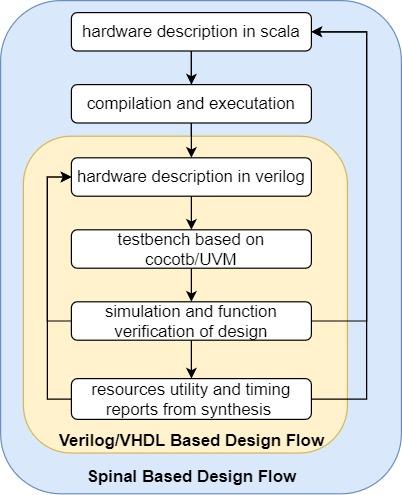
\includegraphics[width=0.4\textwidth]{design_flow.jpg}
\caption{\label{fig:design_flow}SpinalHDL-Based Design Flow.}
\end{figure}


\subsection{Same Description Granularity As Traditional HDLs}
\paragraph{}
Compared with software development, SpinalHDL is to traditional HDLs represented by Verilog what high-level programming languages, such as Java, C/C++ and Python, are to the assembly language. It’s obvious that high-level languages are far more expressive and productive than assembly language and greatly reduce the difficulty of developing a complicated software system like an operating system. Although high-level programming language improves the efficiency of software development, it sacrifices the performance of programs a lot compared to assembly language. 

Similarly SpinalHDL has various advantages over traditional HDLs and it improves the efficiency of designing digital hardware. However, unlike high-level language, it eases and expedites the design process without sacrificing the performance and resources utility of generated hardware. SpinalHDL has almost the same level of precision or granularity of description as traditional HDLs like Verilog or VHDL. It can control the amount of registers and the length of logical path between registers finely. The best proof of approximate description granularity is that for all RTL-level syntax elements in Verilog/VHDL, SpinalHDL has a counterpart. To make it clear, we show all basic elements of RTL level description in Figure 2 and list the mappings from \textbf{SpinalHDL} to \textbf{Verilog} in Table 1.

As shown in Figure 2, RTL-level description, which is the formal definition of a synchronous digital system with one or more clock domains, consists of just five parts basically:
\begin{itemize}
\item clock domains.
\item combinational parts denoted as f(x) in Fig 2.
\item sequential parts, generally speaking, registers and memories, denoted as DFF in Fig 2
\item signals and connections denoted as wires(signal) in between blocks in Fig 1.
\item I/O(interface).
\end{itemize}

\begin{figure}[hbt]
\centering
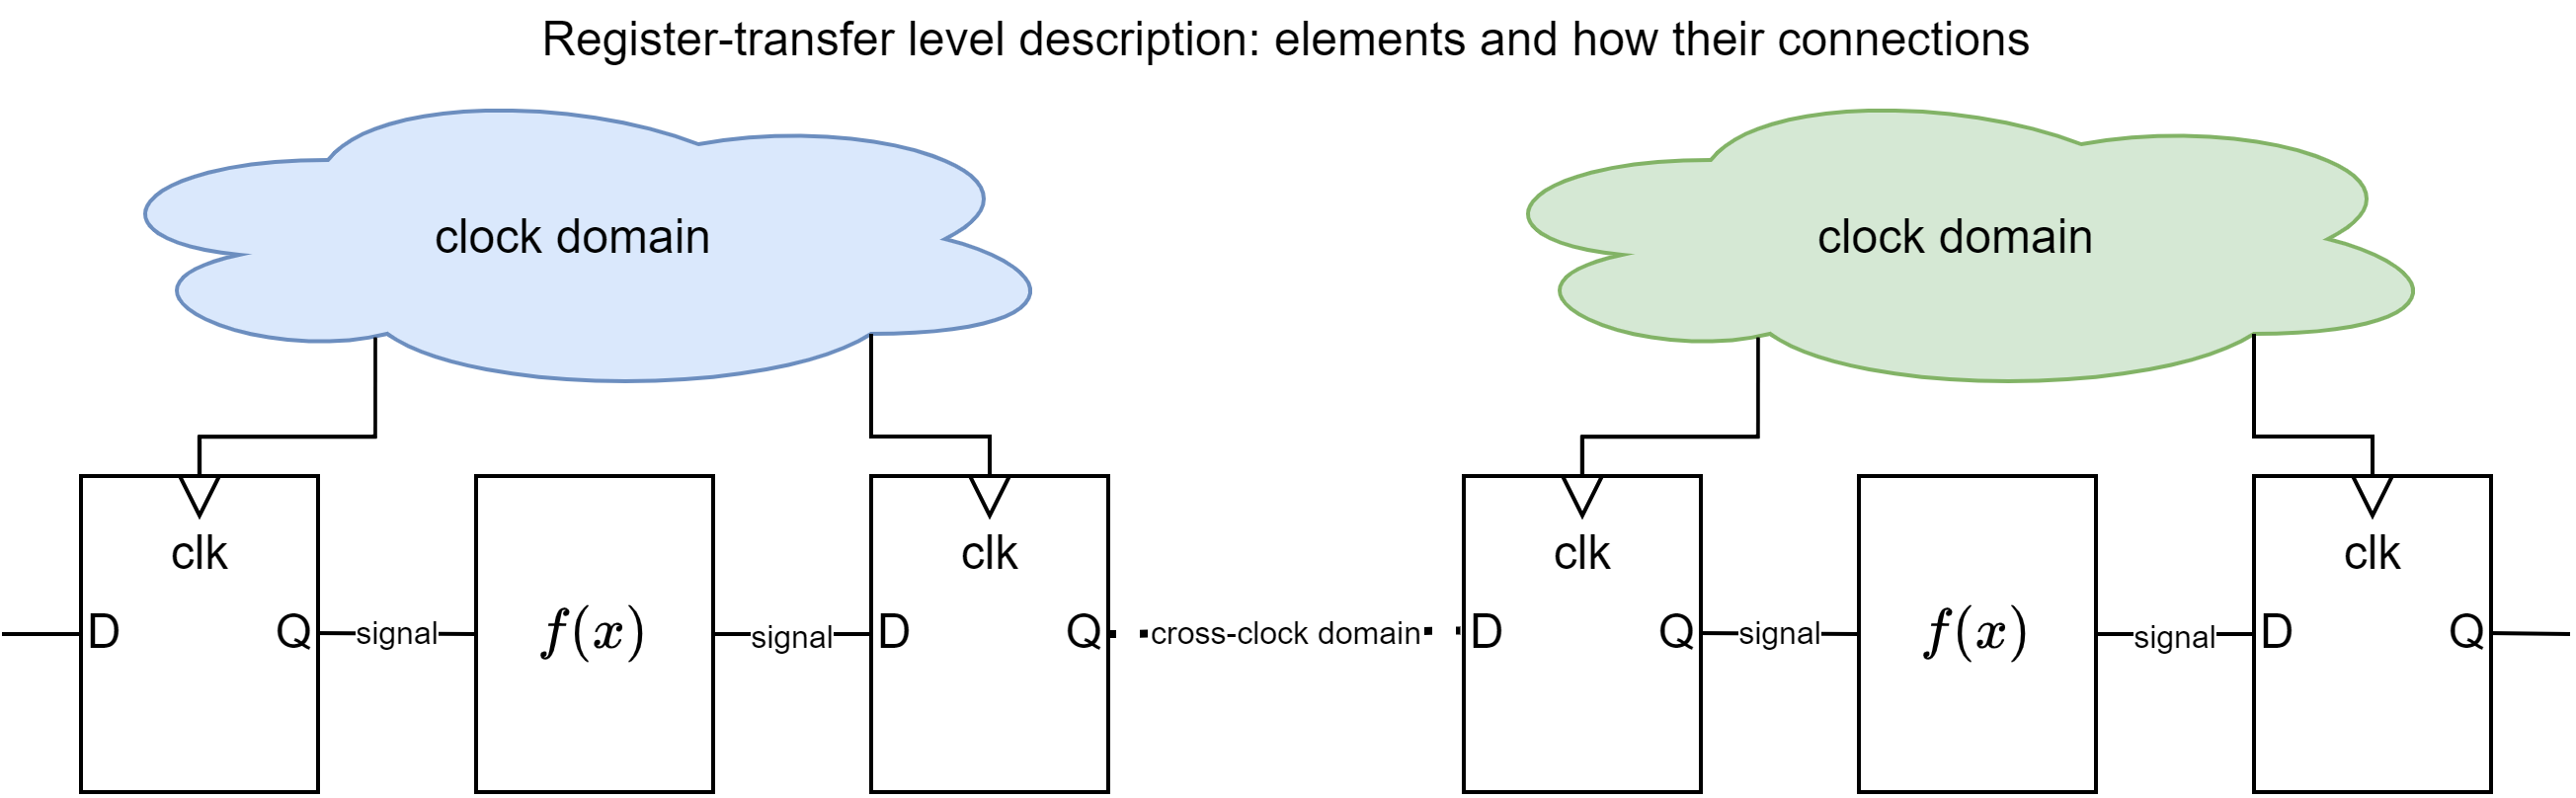
\includegraphics[width=0.8\textwidth]{RTL_element.png}
\caption{\label{fig:RTL_element}Elements In RTL-level Description.}
\end{figure}

For each of these five parts, SpinalHDL provides complete same description capabilities, listed in Table 1. For the worst-case, especially sometimes for beginners, you can use SpinalHDL as Verilog/VHDL with a different set of keywords. And fears of performance loss because of semantic distortion are unnecessary.

\begin{table}[hbt]
\centering
\begin{tabular}{l|l|l}
SpinalHDL elements                      & System Verilog element           & category                \\\hline
in/out                               & input/output                      & I/O                     \\
Bundle                               & interface                         & I/O                     \\
ClockDomain                          & sensitivity list and always block & clock domain            \\
signals(Bool,Bits,UInt,Sint and Vec) & wire/reg/logic and its modifiers  & signals and connections \\
connection(:=)                       & assignment(=, \textless{}=)       & signals and connections \\
when/elseWhen/others                 & if/else if/else                   & combinational           \\
switch/is/default                    & case/default                      & combinational           \\
logical operators                    & logical operators                 & combinational           \\
relational operators                 & relational operators              & combinational           \\
arithmetic operators                 & arithmetic operators              & combinational           \\
registers                            & -                                 & sequential              \\
memories                             & -                                 & sequential             
\end{tabular}
\caption{\label{tab:widgets}Mapping From SpinalHDL To Verilog.}
\end{table}


\subsection{Advantages Of SpinalHDL Over Traditional HDLs}
\subsubsection{Reliability Provided By SpinalHDL}
Using SpinalHDL can greatly increase the reliability of the program and reduce the possibility of bugs, which can reduce the time spent in verification and debugging and expedite the speed of project development. The reliability of codes generated by SpinalHDL comes from:
\paragraph{\textbf{More Accurate Model:}}
For the sequential category of Table 1 including registers and memories, there are no direct syntax elements in Verilog. In fact, for Verilog, implementations of registers ask the synthesis tools to infer the sequential parts by the behaviors of signals in sensitivity lists of \textbf{always} keyword. This awkward idea is shown vividly in Figure 3.

In practice, users of Verilog sometimes encapsulate registers and memories in modules and instantiate them to ensure a proper description. But in SpinalHDL, these have been implemented at the language level. To avoid using confusing \textbf{always} block and sensitivity list, SpinalHDL also describes clock domain and sequential elements directly. At the same time, blocking and nonblocking assignments of Verilog are no longer necessary, the same assignment method":="(which we’d rather call it “connect” or “drive”) could be applied anywhere in SpinalHDL codes.

Besides, SpinalHDL provides a richer type system for signals, which bind types with their behavior. Rather than just be defined by “wire” or “reg” in Verilog, signals can be defined by “Bits”, ”Bool”, “UInt”, ”SInt” and “Vec” in Spinal and have clearer semantics through these more specific definitions. For example, "Bits" and "UInt" both indicate signals with more than one bits, but arithmetic operations can only be applied in "UInt" type and calculations of "Bits" are not allowed. 

\begin{figure}
\centering
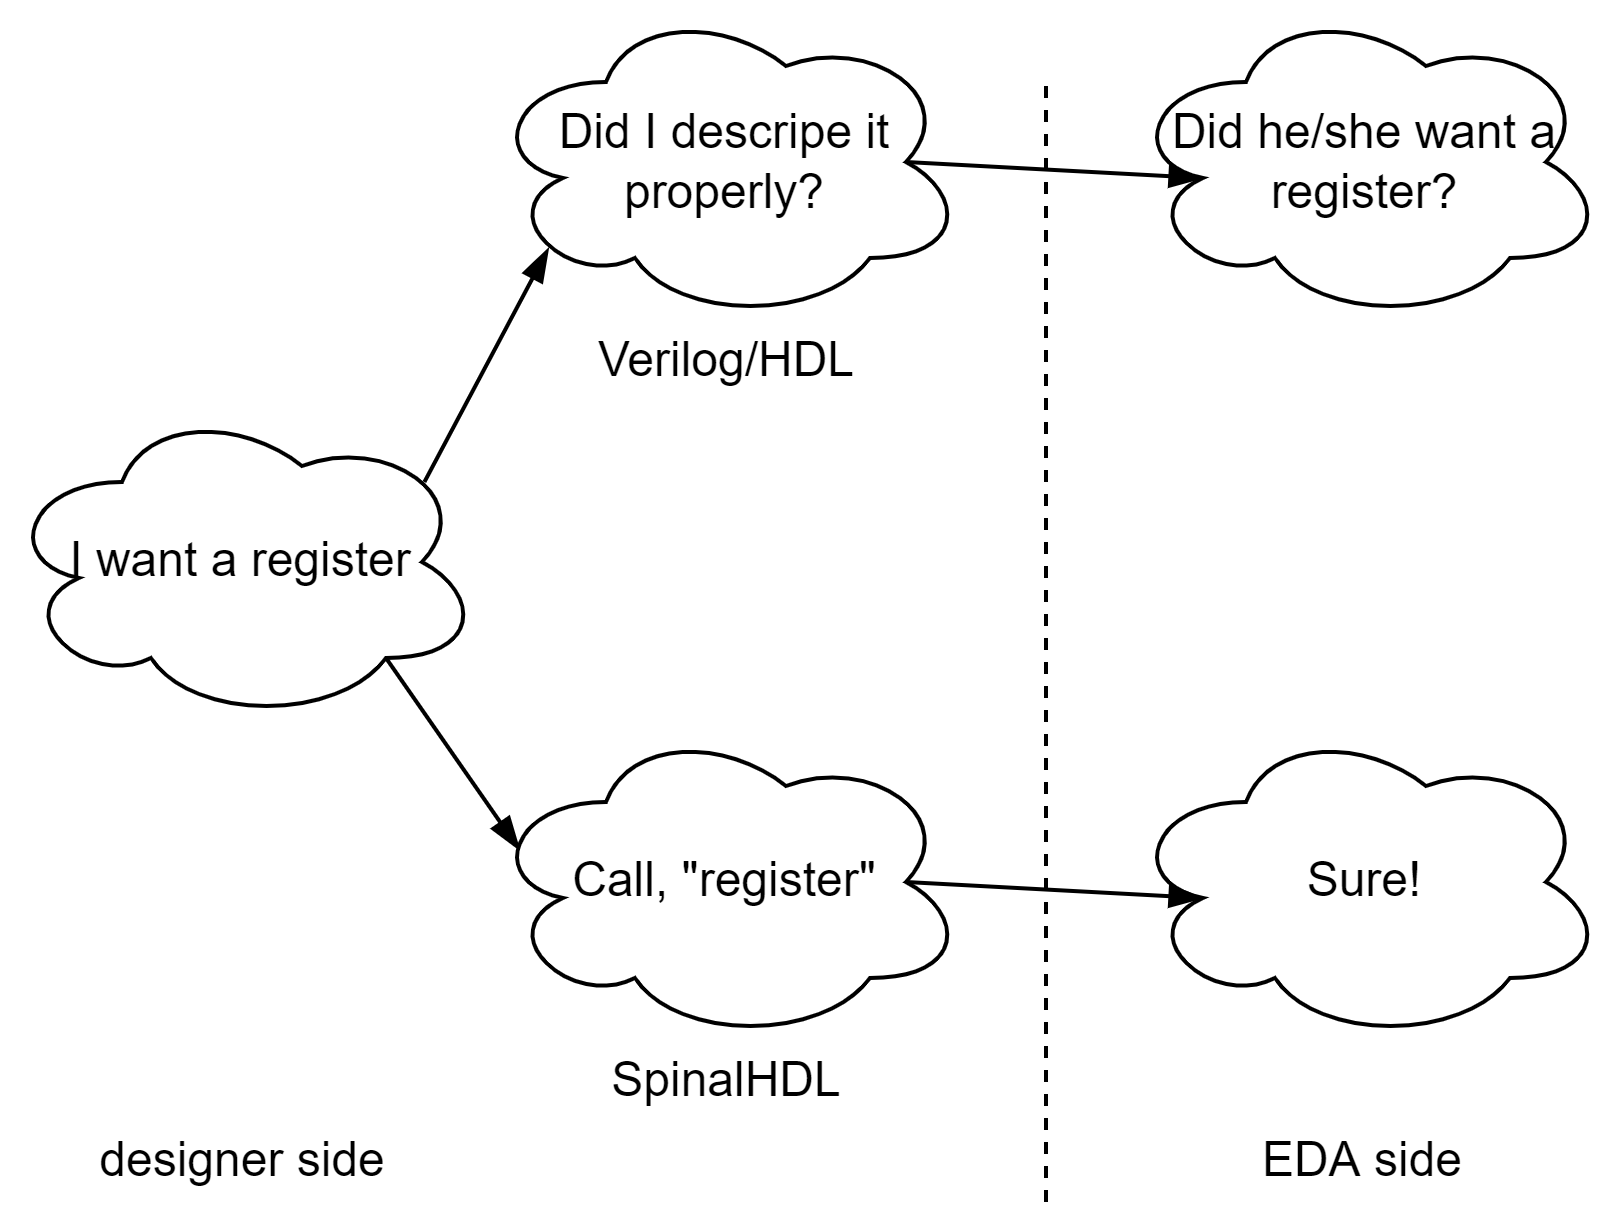
\includegraphics[width=0.55\textwidth]{awkward.png}
\caption{\label{fig:awkward}the awkward design flow of registers in Verilog/VHDL.}
\end{figure}

\paragraph{\textbf{Earlier DRC:}}

With a more accurate model, more design rules could be checked at an earlier stage of the design flow, including:

\begin{enumerate}
\item Semantic problems could be found by the type system, e.g. 'Bits' type in Spinal could not be involved in arithmetic operations.
\item Problems introduced by implicit width expansion or reduction
\item Latches could be found before generating Verilog/VHDL code. As you’ve already “drawn” the diagram describing elements and their connections.
\end{enumerate}

 \paragraph{\textbf{Separate Design Elements And Simulation Elements:}}

Given that Verilog and VHDL are developed initially for simulation and documentation, some of the syntax elements have to play a double role in both design and simulation. For backward compatibility considerations, an “update” on Verilog/VHDL like SystemVerilog could not solve this problem. And it’s prone to confuse synthesizable and unsynthesizable syntax in Verilog especially for beginners. 

An example is the usage of 'if/else'. In Verilog, they are used to model both software-side conditions and hardware-side multiplexers, which makes it sometimes confusing. In SpinalHDL, we use ‘when/ elseWhen / others' to model hardware multiplexers, and thus “free” 'if/else' for expressing software conditions. 

Generally speaking, there’s no such concept called “synthesizable” in SpinalHDL, as long as code can execute and generate Verilog codes, it is naturally “synthesizable”. An exception is the behavior of memories may not be “synthesizable”, which is depenging on the FPGA architecture or process library provided for ASIC.

In summary, with the features above, many design rules of Verilog/VHDL coding became built-in features of the language itself. Thus, designers don't have to deliberately memorize and follow these rules, and as a result, more reliable code could be produced.


\subsubsection{Expressiveness Of SpinalHDL}

\paragraph{\textbf{Advantages In Parametric Design:}}

In Verilog/VHDL, the parametric (and thus, generalized) design is basically implemented by using parameters/generics, however, for complex parametric requirements, it is not enough to only “replace” a series of parameters in the original Verilog/VHDL source. Also, from time to time, instantiating a complex design can be very frustrating.

A typical example is the instantiation template of the Xilinx DSP48E2 slice, which has more than fifty parameters within, making up a huge parameter space, however, only a few of them make sense. On one hand, Defining a design simply by listing these parameters is time-consuming and laborious. On the other hand, because the relationships between parameters are not constrained by a built-in approach (Xilinx has a document of hundreds of pages to describe the constraints), it can be is very error-prone.

Xilinx provides several IPs with corresponding initiation templates to help users configure DSP functions, and at the same time, they also use high-level languages and provide a GUI interface in the process of IP generation. If the slice is described by a generator language like SpinalHDL in the first place, an additional GUI program can be saved, and we can implement the whole project in a more compact way avoiding introducing black boxes(IPs). More specifically, we can design a configuration class in SpinalHDL to manage the individual configuration items and the constraints between them.

\paragraph{\textbf{Software-Hardware Co-Design Ability:}}

Software-hardware co-design is suitable to be applied in the hardware implementation of complicated algorithms. And complex software-hardware co-design requires the flexibility to implement hardware according to the needs of the algorithm. We briefly summarize this collaboration into several situations: 

As shown in Fig 4, in the simplest case, the algorithm determines how the parameters of the hardware are generated.

\begin{figure}[hbt]
\centering
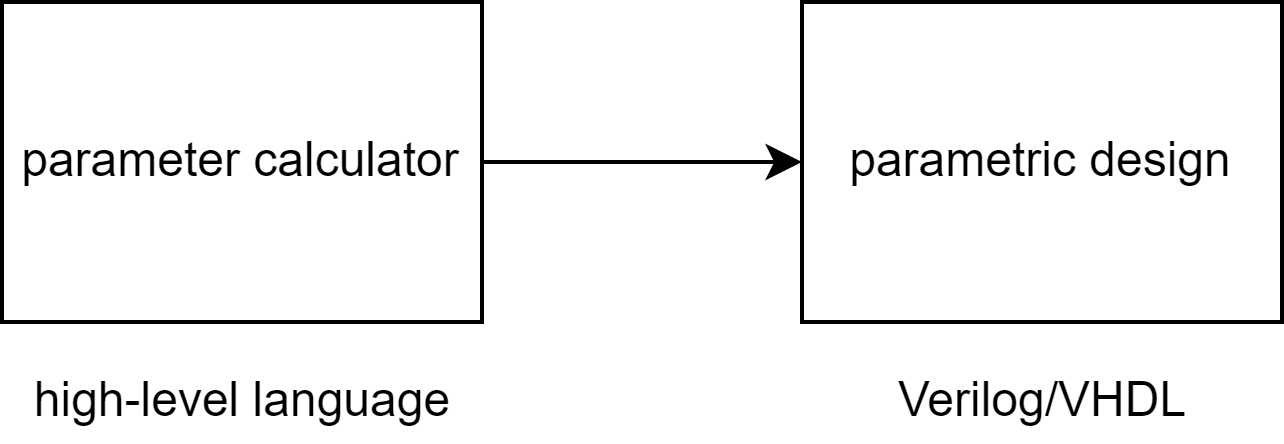
\includegraphics[width=0.5\textwidth]{worst.png}
\caption{\label{fig:worst}the simplest case of software-hardware co-design.}
\end{figure}

In more complex cases, many hardware designs themselves cannot be described directly, but by an algorithm. Examples include various network topologies, parallel algorithms, etc. The algorithm not only determines the parameters of the hardware but also determines which parts the hardware should contain, which parts it should not, and how it should be structured and routed. This requires that our hardware description language can also accommodate more complex algorithms. This degree of collaboration is impossible to achieve only with Verilog with parameters.

In addition, another consideration for hardware design is the parallelism. If there is an efficient parallel algorithm for our application, it is often easy to rewrite the algorithm as a hardware generation algorithm, which will greatly reduce the design time and improve the design reliability. In SpinalHDL, this can be achieved through reliable Scala/Java algorithms from your organization or third-party libraries.

\paragraph{\textbf{Strong Generation Ability:}}

SpinalHDL enables complex hardware generation of algorithms by using features of the Scala language, including:
\begin{enumerate}
    \item Concise and accurate "signal batching" of signals using the collection methods.
    \item Use complex conditions and recursions to handle problems of different sizes.
    \item Reuse existing Scala, or even Java code, to reduce development time and enhance design reliability.
\end{enumerate}

In Figure 5, we give the hardware structure of Benes network as an example to illustrate benefits brought by these features:

\begin{figure}
\centering
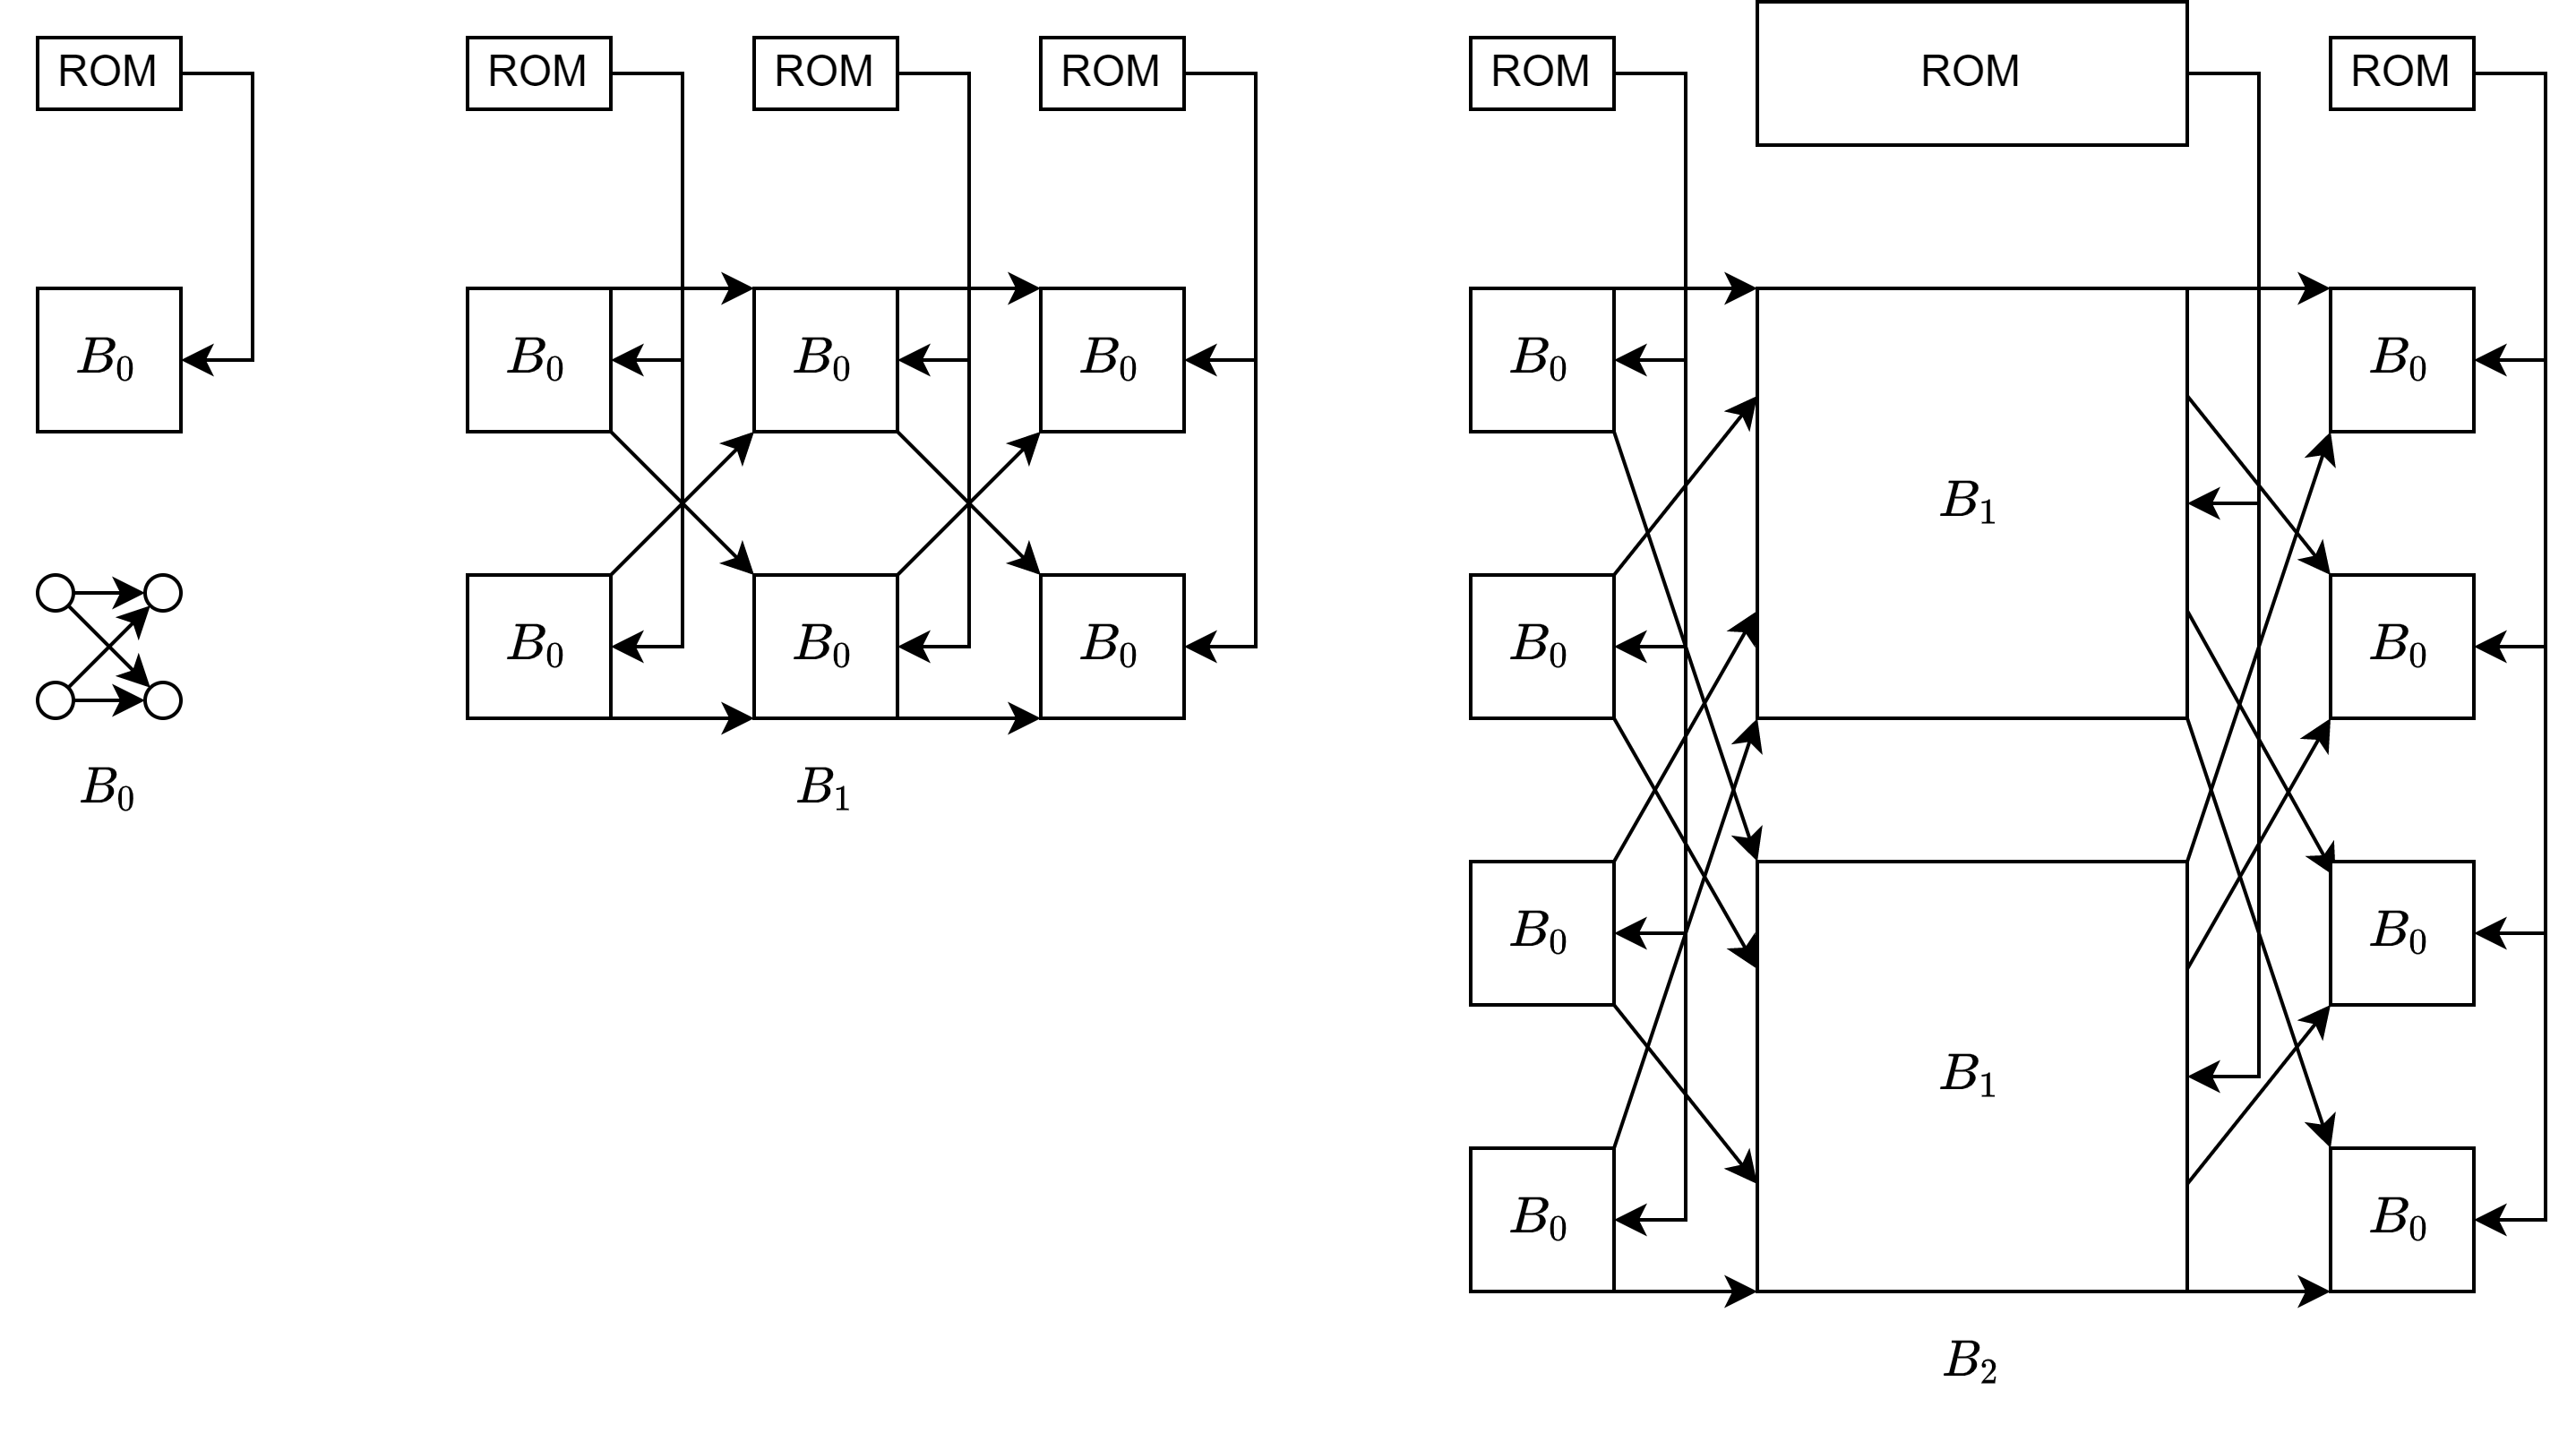
\includegraphics[width=0.55\textwidth]{benes.drawio.png}
\caption{\label{fig:benes}Benes network hardware: switches, routing and control word ROMs.}
\end{figure}


In the design of this hardware, the corresponding specific applications of each language feature mentioned above are specified:
\begin{enumerate}
    \item When describing the blocks of the network topology, we use the collection type "Seq" in Scala and its methods,like "map","zip", and "foreach", to describe connections in a compact way.
    \item With recursion, we provide methods to generate networks of any size.
    \item The generation of Benes network control words is the process of solving a series of 2-coloring problems, and we directly integrate the greedy dyeing algorithm 'org.jgrapht.alg.color.GreedyColoring' in 'JGraphT' (a Java graph theory library) into our SpinalHDL codes to solve this problem.
\end{enumerate}

It is almost impossible to accomplish this design using Verilog/VHDL. But it is common to do so through HCL, because actually, designers are using a high-level language as a Verilog generator not describing the hardware structure directly.

In recent years, domain-specific accelerator design has become an important topic. These tasks are basically expressed in the form of "mapping algorithm implementations to hardware". And these features of SpinalHDL are becoming more and more important because of the convenience they bring to the implementation of complicated algorithms.



\subsubsection{Reusability Of SpinalHDL:}
SpinalHDL also has much better reusability than traditional HDLs, which can improve the efficiency of development greatly. More specifically, you build your own design on the basis of existing high-quality codes more conveniently through better reusability of SpinalHDL. At the same time, your own abilities and experience can be accumulated through gradually building your own code base. Over time, you spend less time on repetitive work and more energy can be spent on valuable problems. And only if the code can be reused at low cost, an open-source hardware community can be formed and grow. The reusability of SpinalHDL mainly comes from the following parts:


\paragraph{\textbf{Good Encapsulations Of Some Basic Design} Elements:}
SpinalHDL itself provides us with good encapsulations of some basic and frequently-used elements, like StateMachine, Stream, Flow and multiple kinds of buses. By using these good encapsulations, you don’t have to build your design from scratch, which can improve your efficiency and reduce the possibility of bugs. 

For example, SpinalHDL provides a convenient abstraction for control path and data path, by modeling them as Stream(s). With stream model, one can view control path and data path as one or more streams from SoC input ports to output ports: (1) the data path of each module within an SoC is to transform the payload data of its input stream(s) and then send to its output ports again as stream(s); (2) as for control path, with the abundant functionalities provided by Spinal HDL to stream model, such as halt/stall, continue, drop, fork, join, etc, one can manipulate the input stream(s) of a module very easily, such as pipelining with back pressure/flow control, retiming, etc. Stream is provided as a class of scala, different manipulation of control path is encapsulated as methods of class. 

Here we take m2sPipe() method of Stream for example, which helps users deal with the error-prone manipulations of valid and ready signals in the pipeline. By using m2sPipe, you can implement piplines with back pressure to slove timing problem more easily. The corresponding hardware structure generated by m2sPipe() is shown in Figure 6:
\begin{figure}[hbt]
\centering
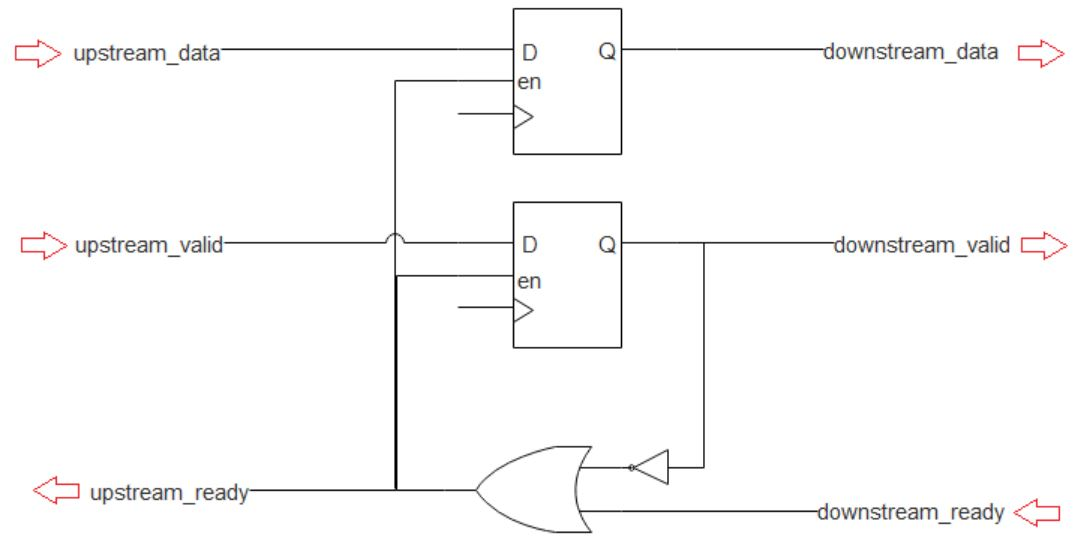
\includegraphics[width=0.55\textwidth]{pipeline.jpg}
\caption{\label{fig:pipeline}Pipeline With Back Pressure}
\end{figure}

Another example is that SpinalHDL provides very good encapsulations for many buses, such as AXI, APB, etc. Especially, AXI is very popular and not easy to implement. SpinalHDL implements AXI interface based on the aforementioned stream model, and provides many useful bus related functionalities, such as crossbar, bus arbiter with/without transaction lock, bus de-mux, bus driver to control registers, etc. And the most important is that the bus interfaces provided by SpinalHDL is error-proof, in that SpinalHDL can check signal types, signal width match, input/output direction, clock domain crossing, etc. With these convenient components provided by SpinalHDL, it facilitates SoC integration to a great extent.

\paragraph{\textbf{Reusability brought by scala language feature:}}

The problems hardware design faces are generally highly customized. But the customization capabilities provided by Verilog/VHDL through parameters/Generics are insufficient, and codes in Verilog is difficult to face many situations. At the same time, Verilog/VHDL's self-interpretation is poor, and in many cases it is difficult to understand and use the source code developed by other people even if it is available. There are two main reasons for the difficulty of understanding codes in traditional HDLs: 1)The description in Verilog/VHDL is too low-level; 2) Design rules used by different teams are inconsistent. 

From the perspective of language features, higher-level and more complex functions of scala allow designs to support more complex generation patterns, resulting in greater generality, making it easier to design truly general-purpose designs for multiple scenarios. Besides scala features of object-oriented and type systems allow developers to describe designs in a higher level and improve program’s capabilities of self-interpretation. For example, with SpinalHDL, we can use “.” to index methods of a class and extend custom types to define various concepts, such as convolution-encoded trellis. From the perspective of community and tools, established communities such as Github provide a natural environment for collaboration and discussion. And Library distribution and package management systems of scala make code acquisition and deployment very easy, such as pypi-pip and maven-sbt.

Besides the reuse of codes, another reuse phenomenon within project team is the reuse of design rules/protocols. What SpinalHDL can provide to this kind of reuse includes:
\begin{enumerate}
    \item Object-oriented systems extend design capabilities:  1) Reuse design through inheritance; 2) Specify design rules via traits of scala
    \item Implicit of scala allows design rules to exist in a global, transparent way, rather than another way
    \item Better IDEs that support remote development also enhance this reuse
\end{enumerate}

In a word, the reusability provided by SpinalHDL is not only achieved through language features, but also through the complete community environment including the IDE tool chain, and the high-level host language



\section{Meta-language Based Construction Of Digital Logic}
\subsection{The Concept Of A Meta-Language Above Circuits}
\paragraph{}
Hardware Construction Languages such as SpinalHDL, Chisel, Migen, and Clash can be thought of as a meta-language layer above circuits, in contrast to traditional HDLs that directly describe the circuit. The meta-language layer enables hardware designers to focus more on the semantics of the circuits, rather than the concrete structure, and makes it easier for both programs and humans to reason about the correctness of a design.

\begin{figure}[hbt]
\centering
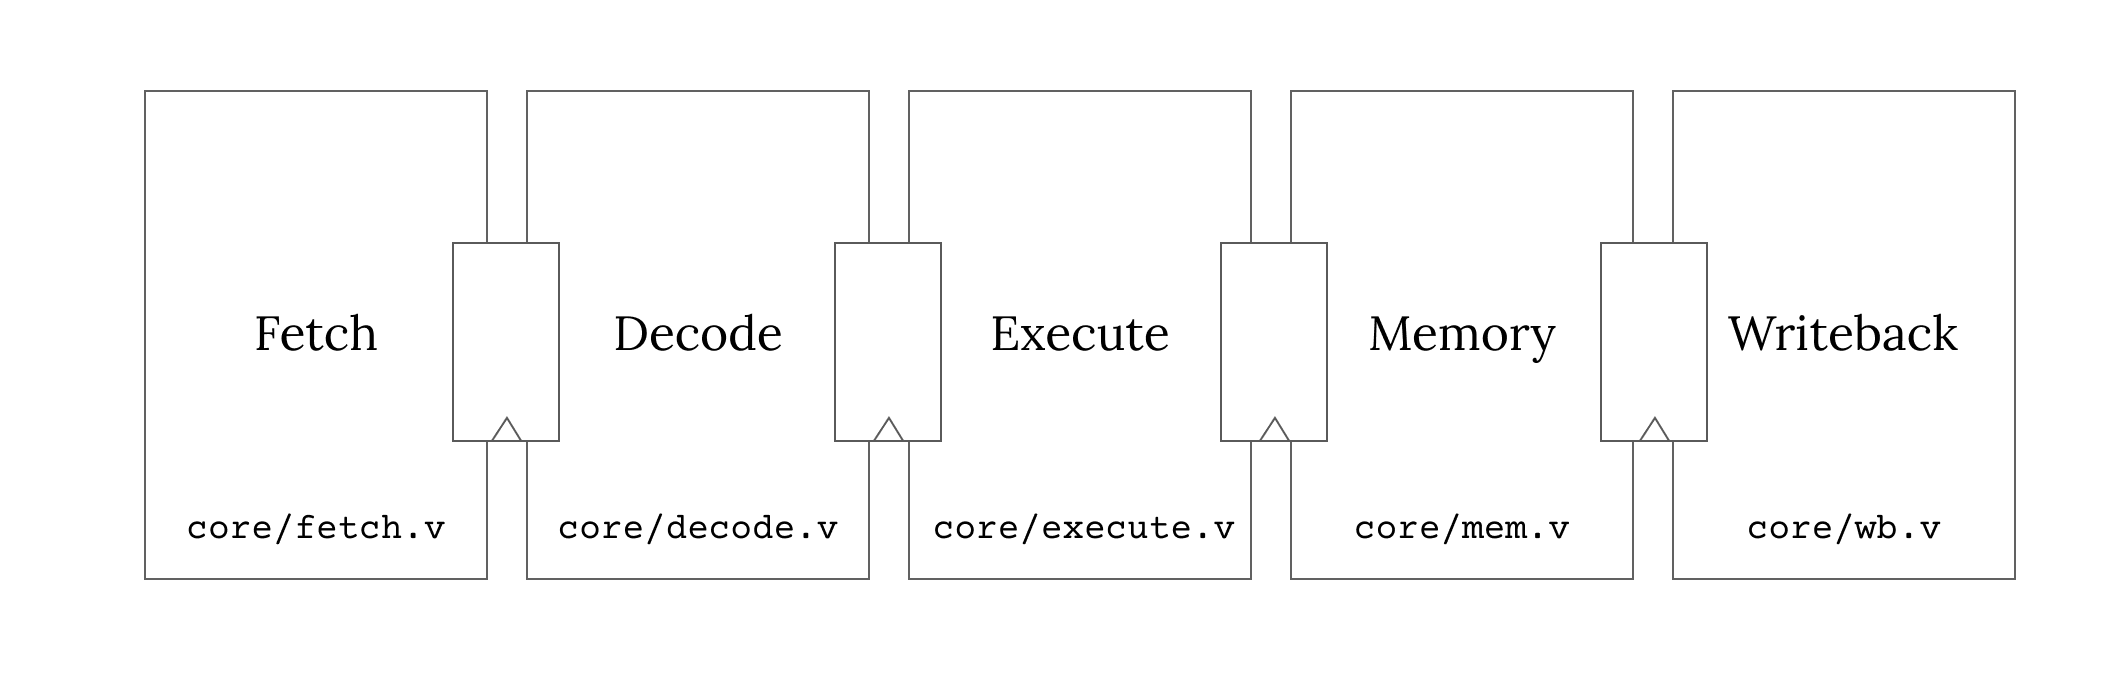
\includegraphics[width=0.65\textwidth]{Frame_1(1).png}
\caption{\label{fig:frame1} a classical RISC pipeline consists of the Fetch, Decode, Execute, Memory, and Writeback stages.}
\end{figure}

\begin{figure}
\centering
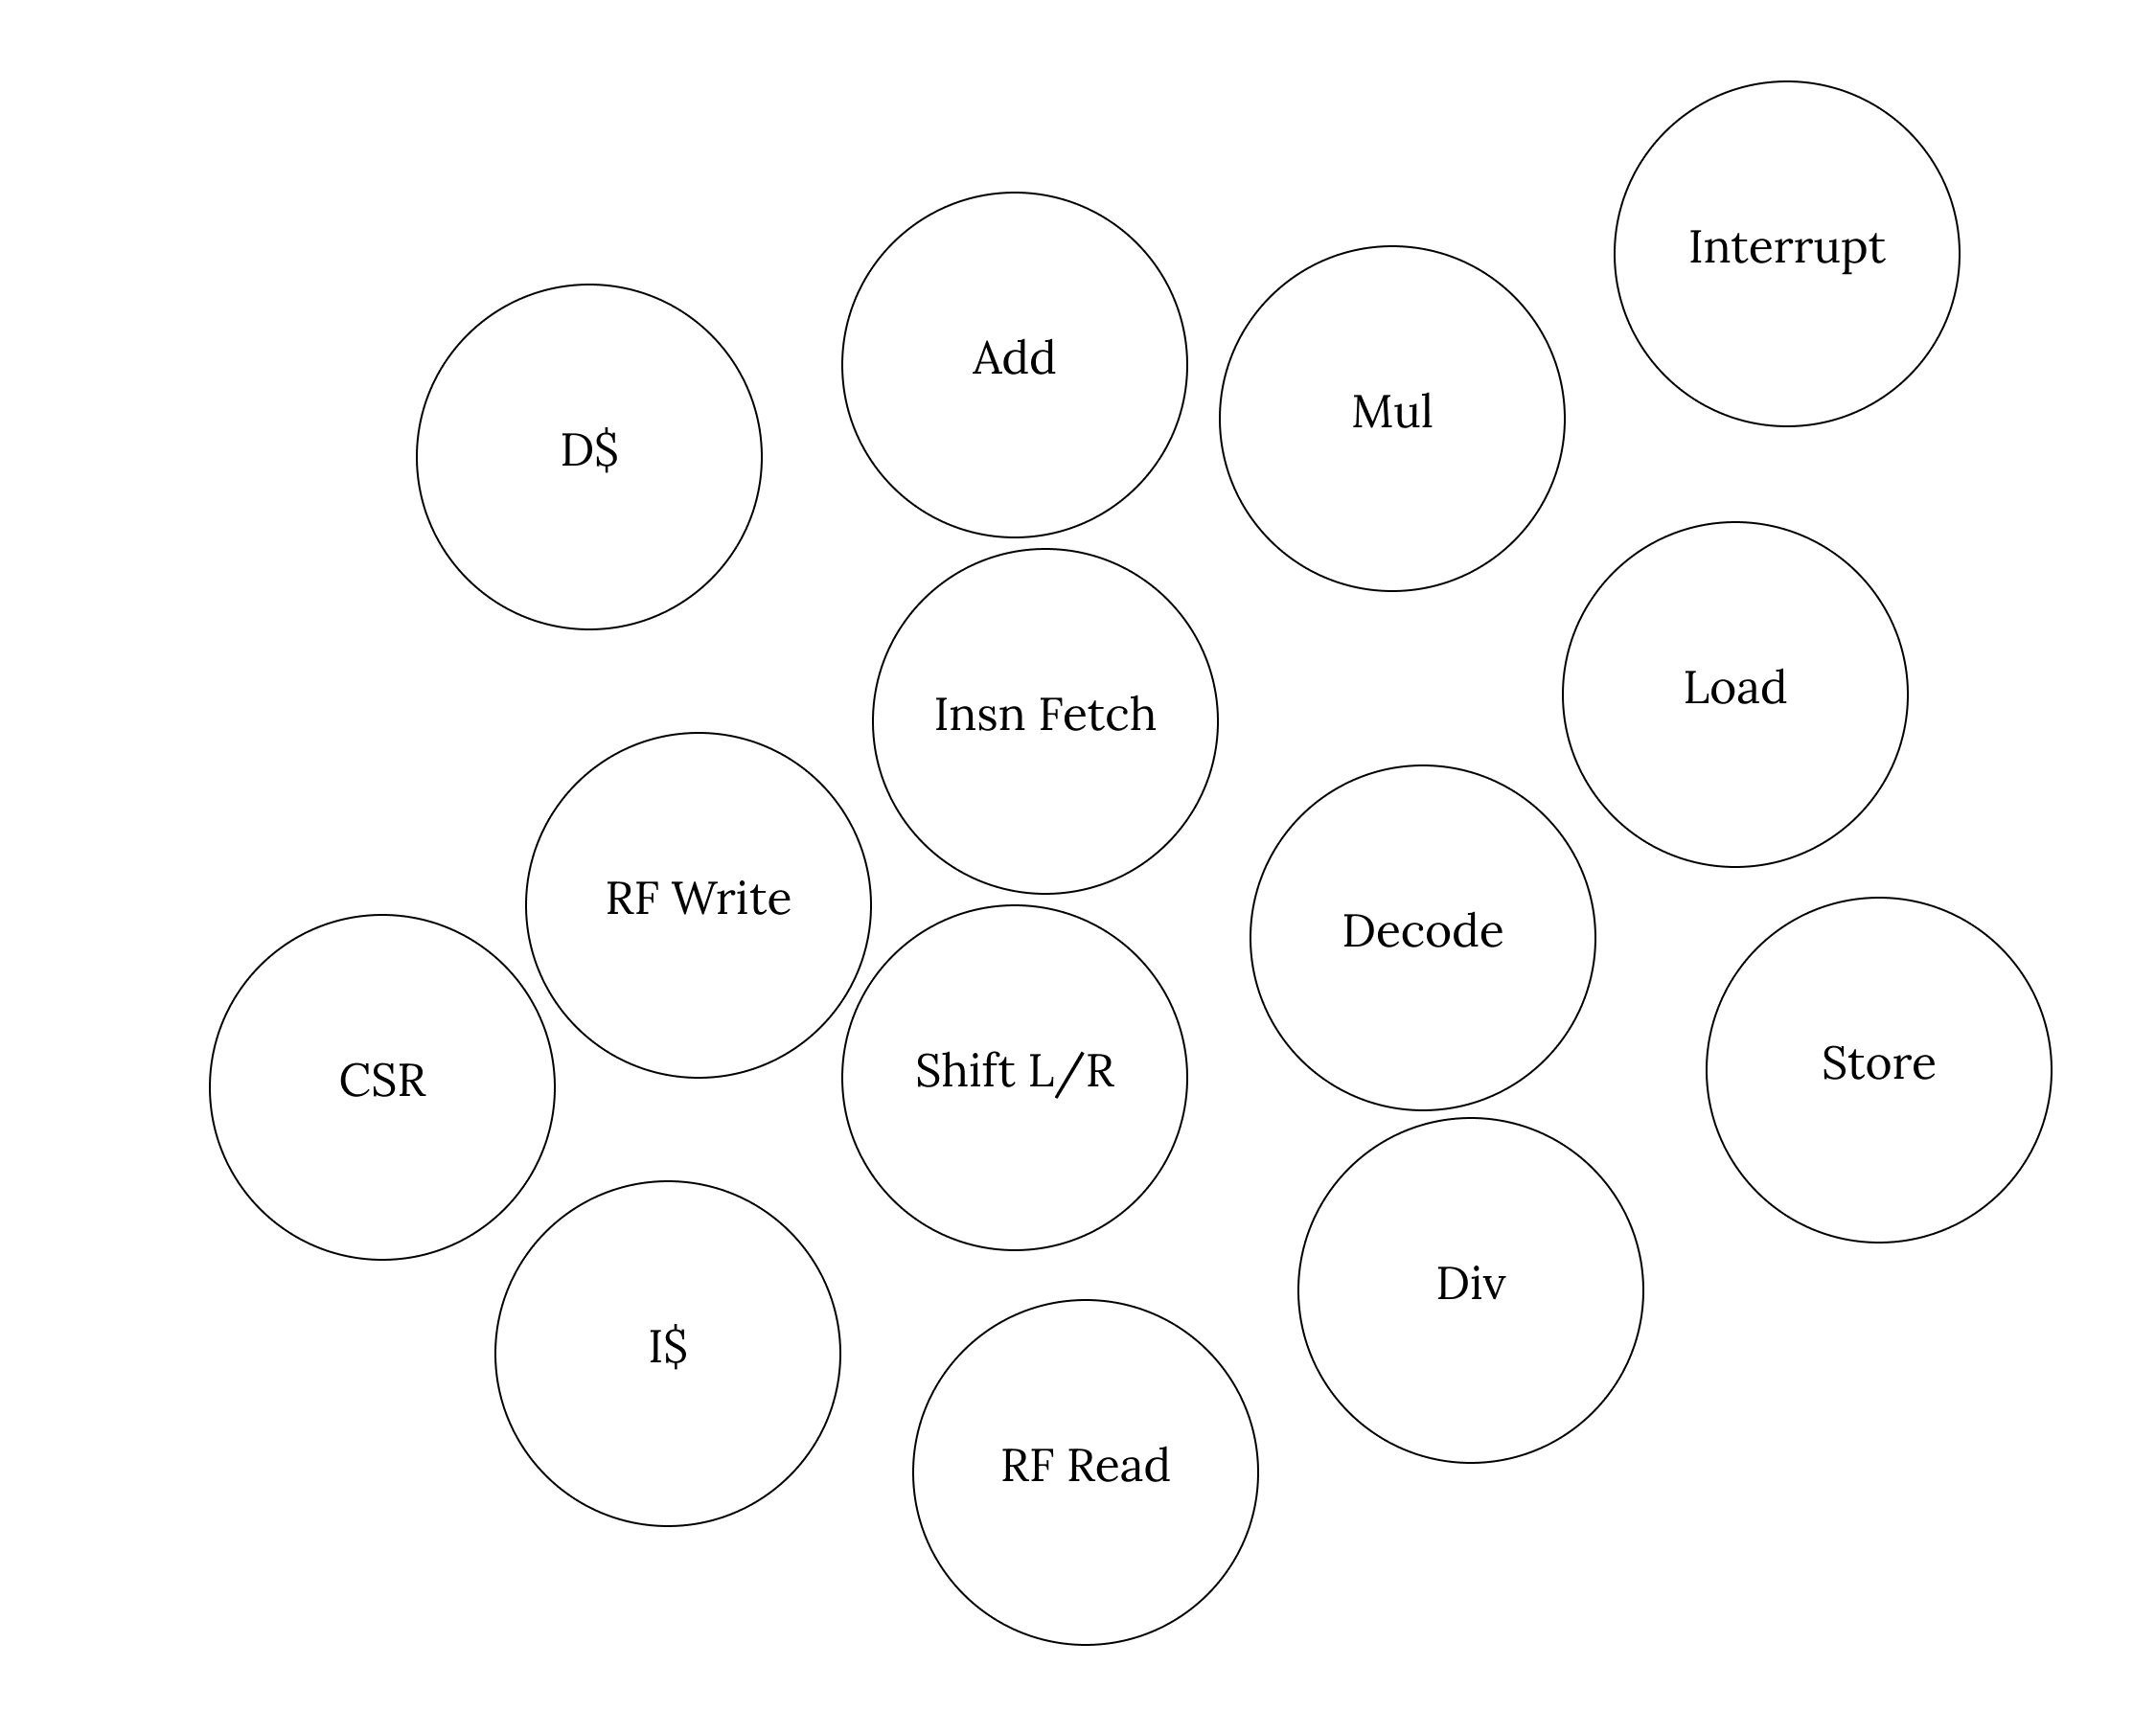
\includegraphics[width=0.6\textwidth]{Frame_1(2).png}
\caption{\label{fig:frame3}From a semantic perspective, a classical RISC pipeline consists of register file access, cache access, instruction fetch/decode, arithmetic operation, and other functions.}
\end{figure}

The problem with the traditional structural approach of hardware design is that it does not match the functional specification of the circuit. For example, to efficiently add a multiplication function to a classical 5-stage RISC pipeline optimized for FPGAs, which is shown in Fig7, the corresponding logic has to be implemented separately in the Decode, Execute, Memory, and Writeback stages, since hardware multipliers on FPGAs usually have a latency longer than 1 cycle. As shown in Fig 8, A nicer abstraction is demonstrated by the VexRiscv project implemented in SpinalHDL: semantically-specified functions are decoupled from the pipeline structure with a Plugin approach, where functions are implemented in their own Scala modules and plug themselves into the pipeline during netlist generation.

\textbf{Deeply-embedded and shallowly-embedded HCLs:}

There are two classes of hardware construction languages: deeply-embedded and shallowly-embedded. Widely-used shallowly-embedded HCLs include SpinalHDL, Chisel, and Migen, while Clash is a leading deeply-embedded HCL.

\subsection{Advanced Type Systems For Hardware Design}
The type systems of traditional hardware description languages such as Verilog, SystemVerilog, and VHDL are quite limited in terms of expressiveness and strength of constraints:
\begin{itemize}
    \item There are only plain old product types with no constraints on the usage of the type constructor, and there is no support for sum types.
    \item There is only trivial support for polymorphism.
    \item There are no higher-order types.
\end{itemize}

Meanwhile, most modern hardware construction languages have access to an advanced type system with both sum and product types, parametric polymorphism, and higher-order types.


\textbf{Sum types, product types, and private type constructors: }

A product type, known as a struct in most programming languages, is a data structure that holds zero or more values of different types. In SpinalHDL product types are used to represent a 'Bundle' of signals, for example:

\begin{lstlisting}[language=scala]
val io = new Bundle {
  val memWrite = slave  Flow(MemoryWrite())
  val cmdA     = slave  Stream(UInt(8 bits))
  val cmdB     = slave  Stream(Bits(32 bits))
  val rsp      = master Stream(Bits(32 bits))
}
\end{lstlisting}

A sum type, also known as a tagged union, is a data structure that can hold a single value from one of a fixed number of different types and retains the type of the value held.

Though neither Verilog nor traditional software programming languages such as C have direct support for sum types, we can emulate its behavior in C:

\begin{lstlisting}[language=C]
struct S {
  int tag;
  union {
    int variant1;
    char *variant2;
  };
};

//Now we can check tag and use either variant1 or variant2 accordingly.
\end{lstlisting}

A simple yet well-known example of a sum type is the 'Option' type:

\begin{lstlisting}
// Define the parameterized type Option.
// sealed means that subclasses of Option can only be defined in the same file,
// making it a sum type.
sealed abstract class Option[T]

// Define two subclasses of 'Option[T]' as sum type variants.
case class Some[T](x: T) extends Option[T]
case object None extends Option[Nothing]
\end{lstlisting}

\begin{table}[hbt]
\centering
\begin{tabular}{l|l|l}
Language & Sum Type & Product Type\\\hline
C        & struct S { int tag; union { ... }; }; & struct S { ... };\\
Scala    & sealed abstract class Option[T]       & class C { ... } \\
Scala    & data Maybe a = Nothing | Just a       & data Prod = ProdCons { .. }
\end{tabular}
\caption{\label{tab:widgets}Mapping From SpinalHDL To Verilog.}
\end{table}

With the presence of sum and product types, it’s possible to place constraints on the set of representable values. For instance, in a deeply-embedded HCL, a data signal gated by a `VALID` signal can be represented using an `Option` type, making it impossible to read the value without checking that `VALID` is `high`.

In a shallowly-embedded HCL sum types can only be used on circuit structure but not data, but we can still simulate the behavior of `Option[T]` using the newtype pattern. We create a function:

\begin{lstlisting}[language=scala]
readSignal[T](value: DynamicOption[T], 
             onSome: T => Unit, 
             onNone: () => Unit):Unit = {
  when(value.valid) {
    onSome(value.data)
  }
  when(!value.valid) {
    onNone()
  }
}
\end{lstlisting}
that selects either onSome or onNone depending on value. With the DynamicOption type constructor being private, it is sufficient to protect value from unintended access without checking VALID.

\textbf{Subtyping and parametric polymorphism: }

Subtyping, whose most common form is inheritance, is a mechanism to build hierarchies of types. 

Parametric polymorphism, also known as generics, is a mechanism to write type-level functions that take types as input and produces a monomorphic type or function as an output.

\begin{lstlisting}[language=scala]
def isGreaterThan[T](left: T, 
                    right: T)(implicit order: Ordering[T]): Boolean
  = order.gt(left, right)
\end{lstlisting}

\subsection{Beyond SpinalHDL}
SpinalHDL successfully utilized a lot of constructs in Scala to improve the efficiency of the hardware design process, but there are more possibilities in abstracting properties out of hardware and verifying them during compilation time. In this section, we introduce various approaches from different software programming languages that we think can benefit hardware designing too.

\textbf{Type-level natural numbers:}

It is well-known that natural numbers can be encoded as types and computations can be performed on it. For example, as shown in Fig 9, a n-level arbitration tree with a fanout factor of m can be described using the following Clash type:

\begin{lstlisting}[language=Haskell]
arbitrationTree ::
  HiddenClockResetEnable dom =>
  KnownNat n, m =>
  Signal dom (Vec (m ^ n) (Maybe a)) ->
  Signal dom (Maybe a)

arbitrationLayer ::
  HiddenClockResetEnable dom =>
  KnownNat m =>
  Signal dom (Vec m (Maybe a)) =>
  Signal dom (Maybe a)
\end{lstlisting}

\begin{figure}
\centering
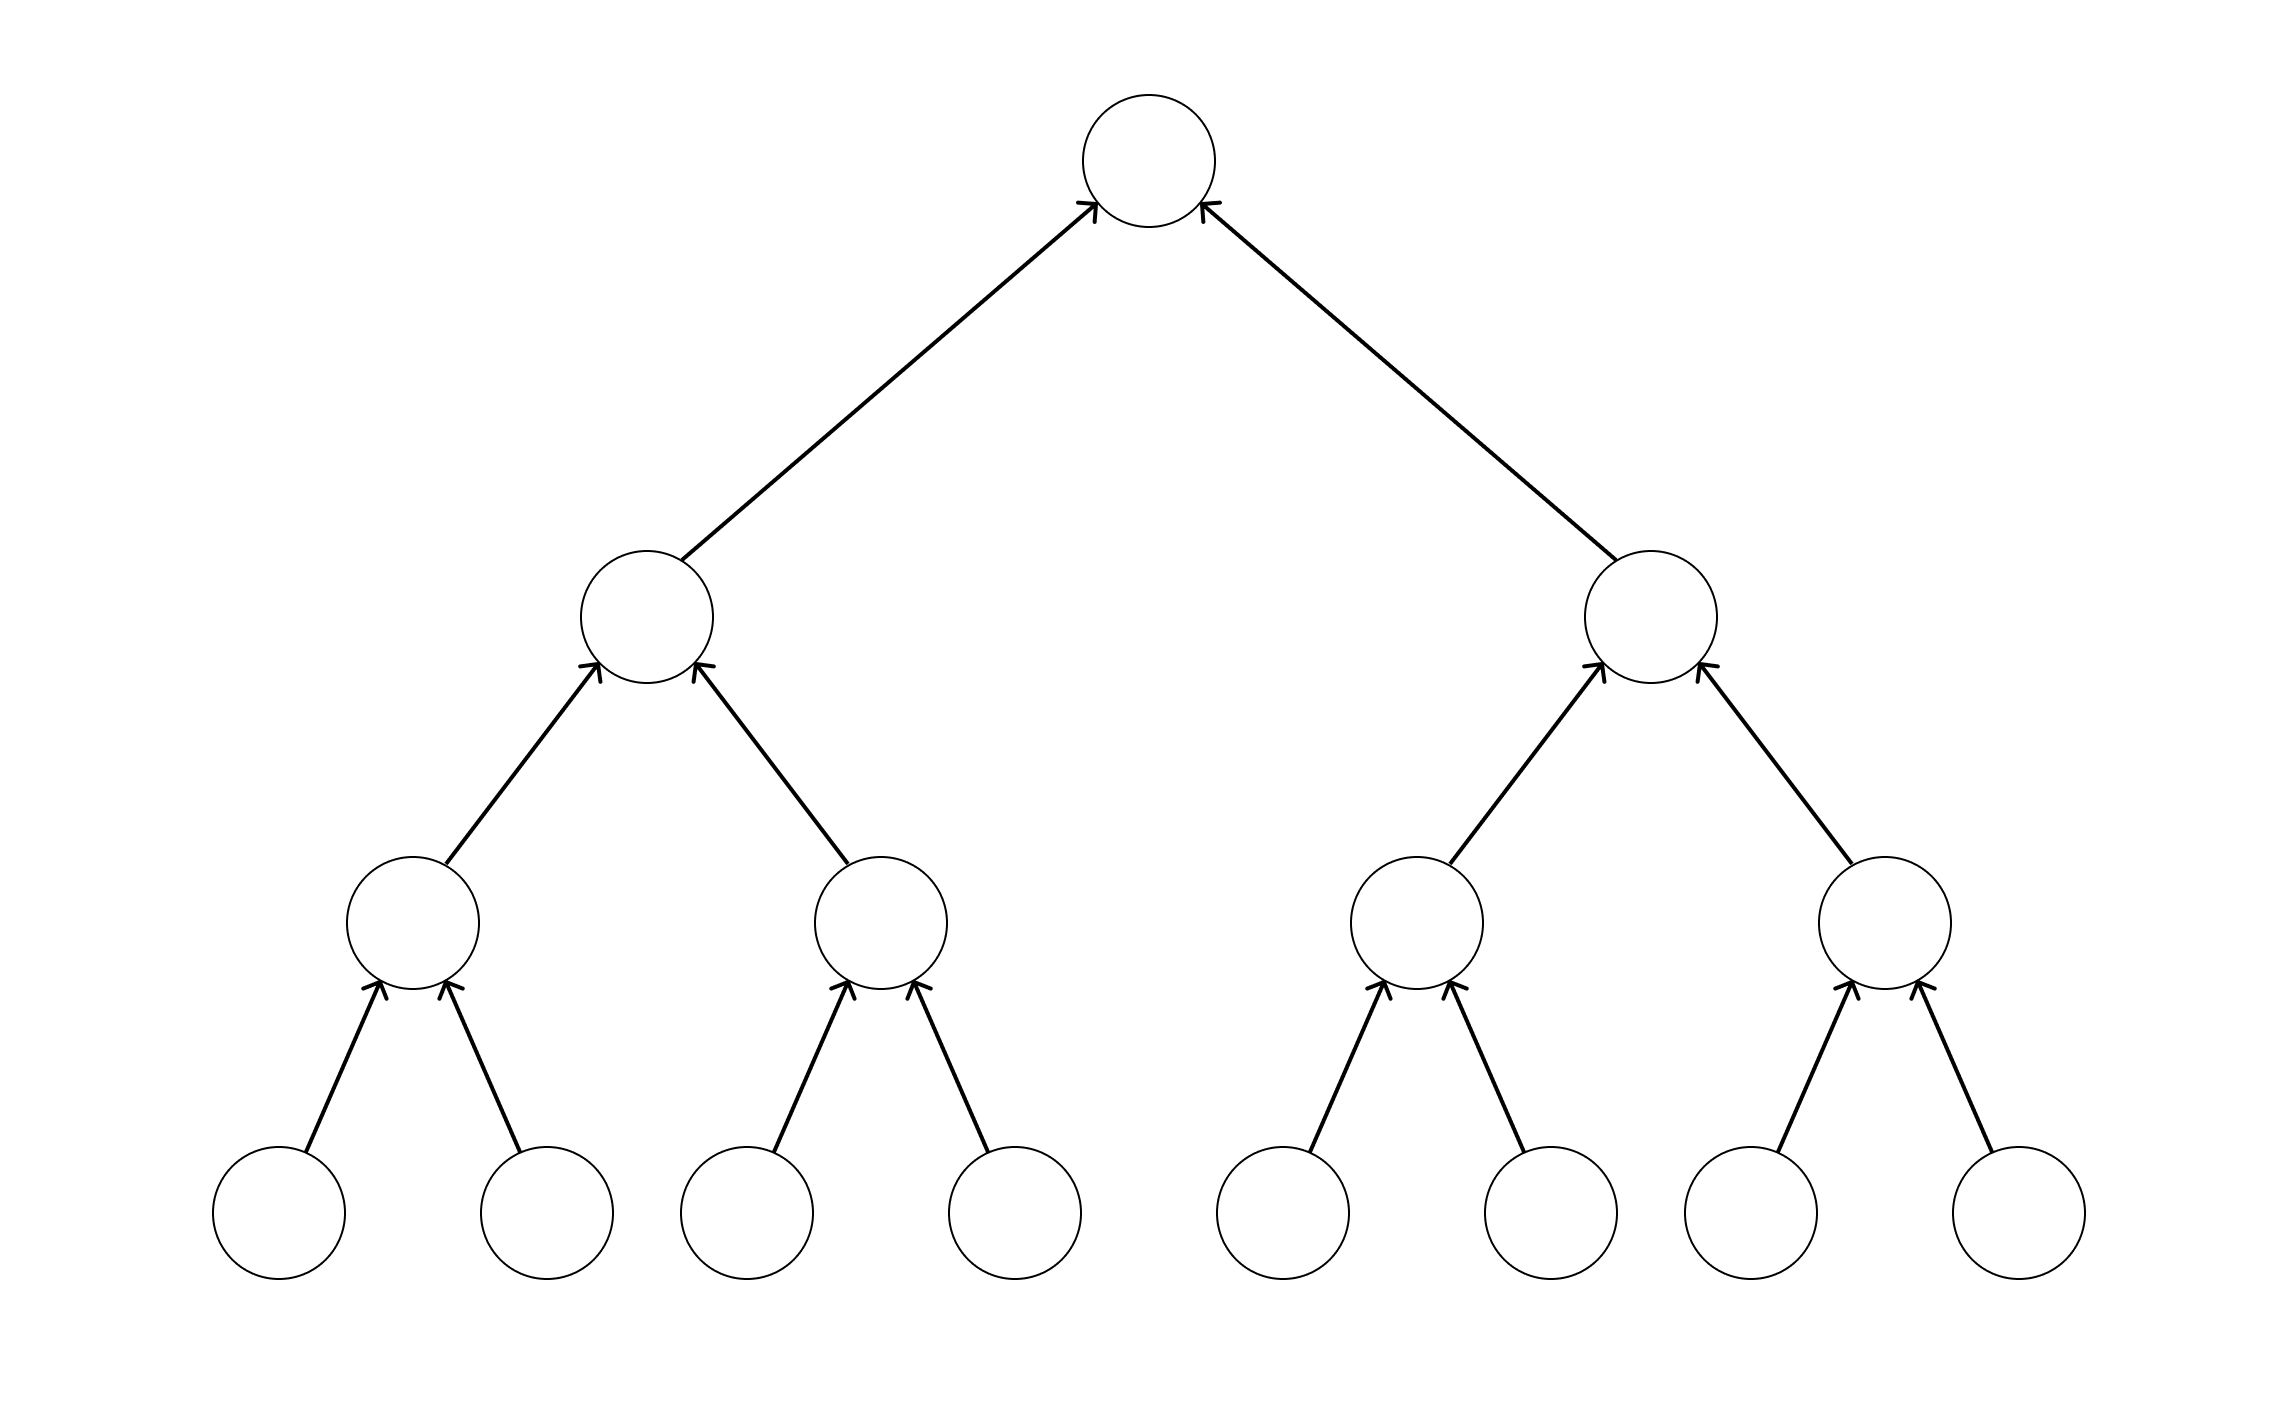
\includegraphics[width=0.6\textwidth]{Frame_1(6).png}
\caption{\label{fig:frame6}A 8-way, 3-stage arbitration tree. n = 3, m = 2.}
\end{figure}

Generic parameters are implicitly a 'forall' constraint, requiring the implementation to be valid for all values of 'n' and 'm'. An implementation that fails to satisfy the type signature is almost always incorrect and is reported as a compile-time error.

A major benefit of the implied 'forall' constraint on generic parameters including type-level natural numbers is that it prevents confusion of constants that “accidentally” have the same value. As shown in Fig 10, An example is matching all entries in a buffer with another 'n' buffers of size 'm':

\begin{figure}[hbt]
\centering
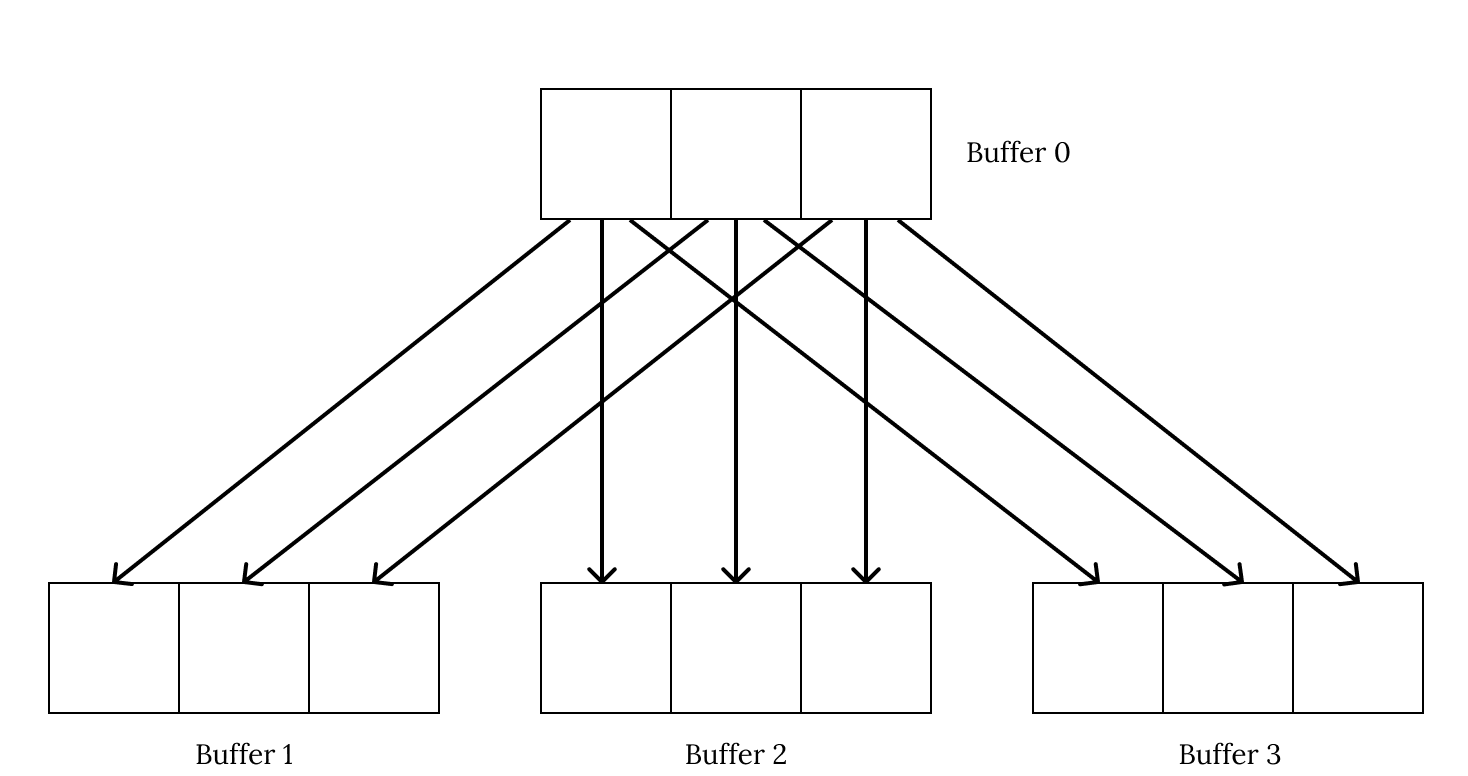
\includegraphics[width=0.6\textwidth]{Frame_1(5).png}
\caption{\label{fig:frame6}match all entries in a buffer with another 'n' buffers of size 'm'}
\end{figure}

Let’s consider the family of configurations where n = m. For HCLs without type-level natural number support such as SpinalHDL, confusing n and m somewhere in the design will not be reported as an error during either compilation or Verilog generation - but the logic will be silently incorrect. But for Clash where type-level natural number is extensively integrated into hardware primitives such as Vec and BitVector, the compiler will ensure that the logic passes type checking for all values of n and m - not just the values defined in the configuration.

\textbf{Refinement types:}

A refinement type is a type endowed with a predicate that specified which values from the original types should be an element of the refined type. For hardware design, refinement types can be used to pass down the properties of a signal. An example is a fixed-point arithmetic unit. In some cases, we would like to restrict the range of the signal on the input side (like restricting the value of an 8-bit signal to 0-200), and validate that the output signal satisfies certain constraints (for example, a circuit that multiplies the input of range 0-200 by 2 should have a value domain of 0-400). With refinement types, we are able to refine the input type with an explicit range and have an SMT solver check the output signal’s properties for us.

\subsection{The Compilation Flow Of HCLs}
A digital design encoded as a program in a Hardware Construction Language needs to be compiled to a synthesizable description of the circuit. With all major commercial and open-source synthesis toolchains supporting Verilog as a first-class source language, it’s a natural choice for HCLs to use Verilog as a compilation target, and delegate backend processes to the synthesis toolchain.

As shown in Fig 10, for shallowly-embedded HCLs, the compilation flow consists of 3 steps:
\begin{enumerate}
    \item Type-checking and *software* compilation.
    \item IR generation.
    \item IR-to-Verilog code generation.
\end{enumerate}

Deeply-embedded HCLs have a slightly different compilation flow:
\begin{enumerate}
    \item Type-checking and *IR* compilation.
    \item IR-to-Verilog code generation. (* some deeply-embedded HCL, like Clash, can also be compiled by a software-targeting compiler to an executable program that simulates the behavior of the circuit)
\end{enumerate}

\begin{figure}[hbt]
\centering
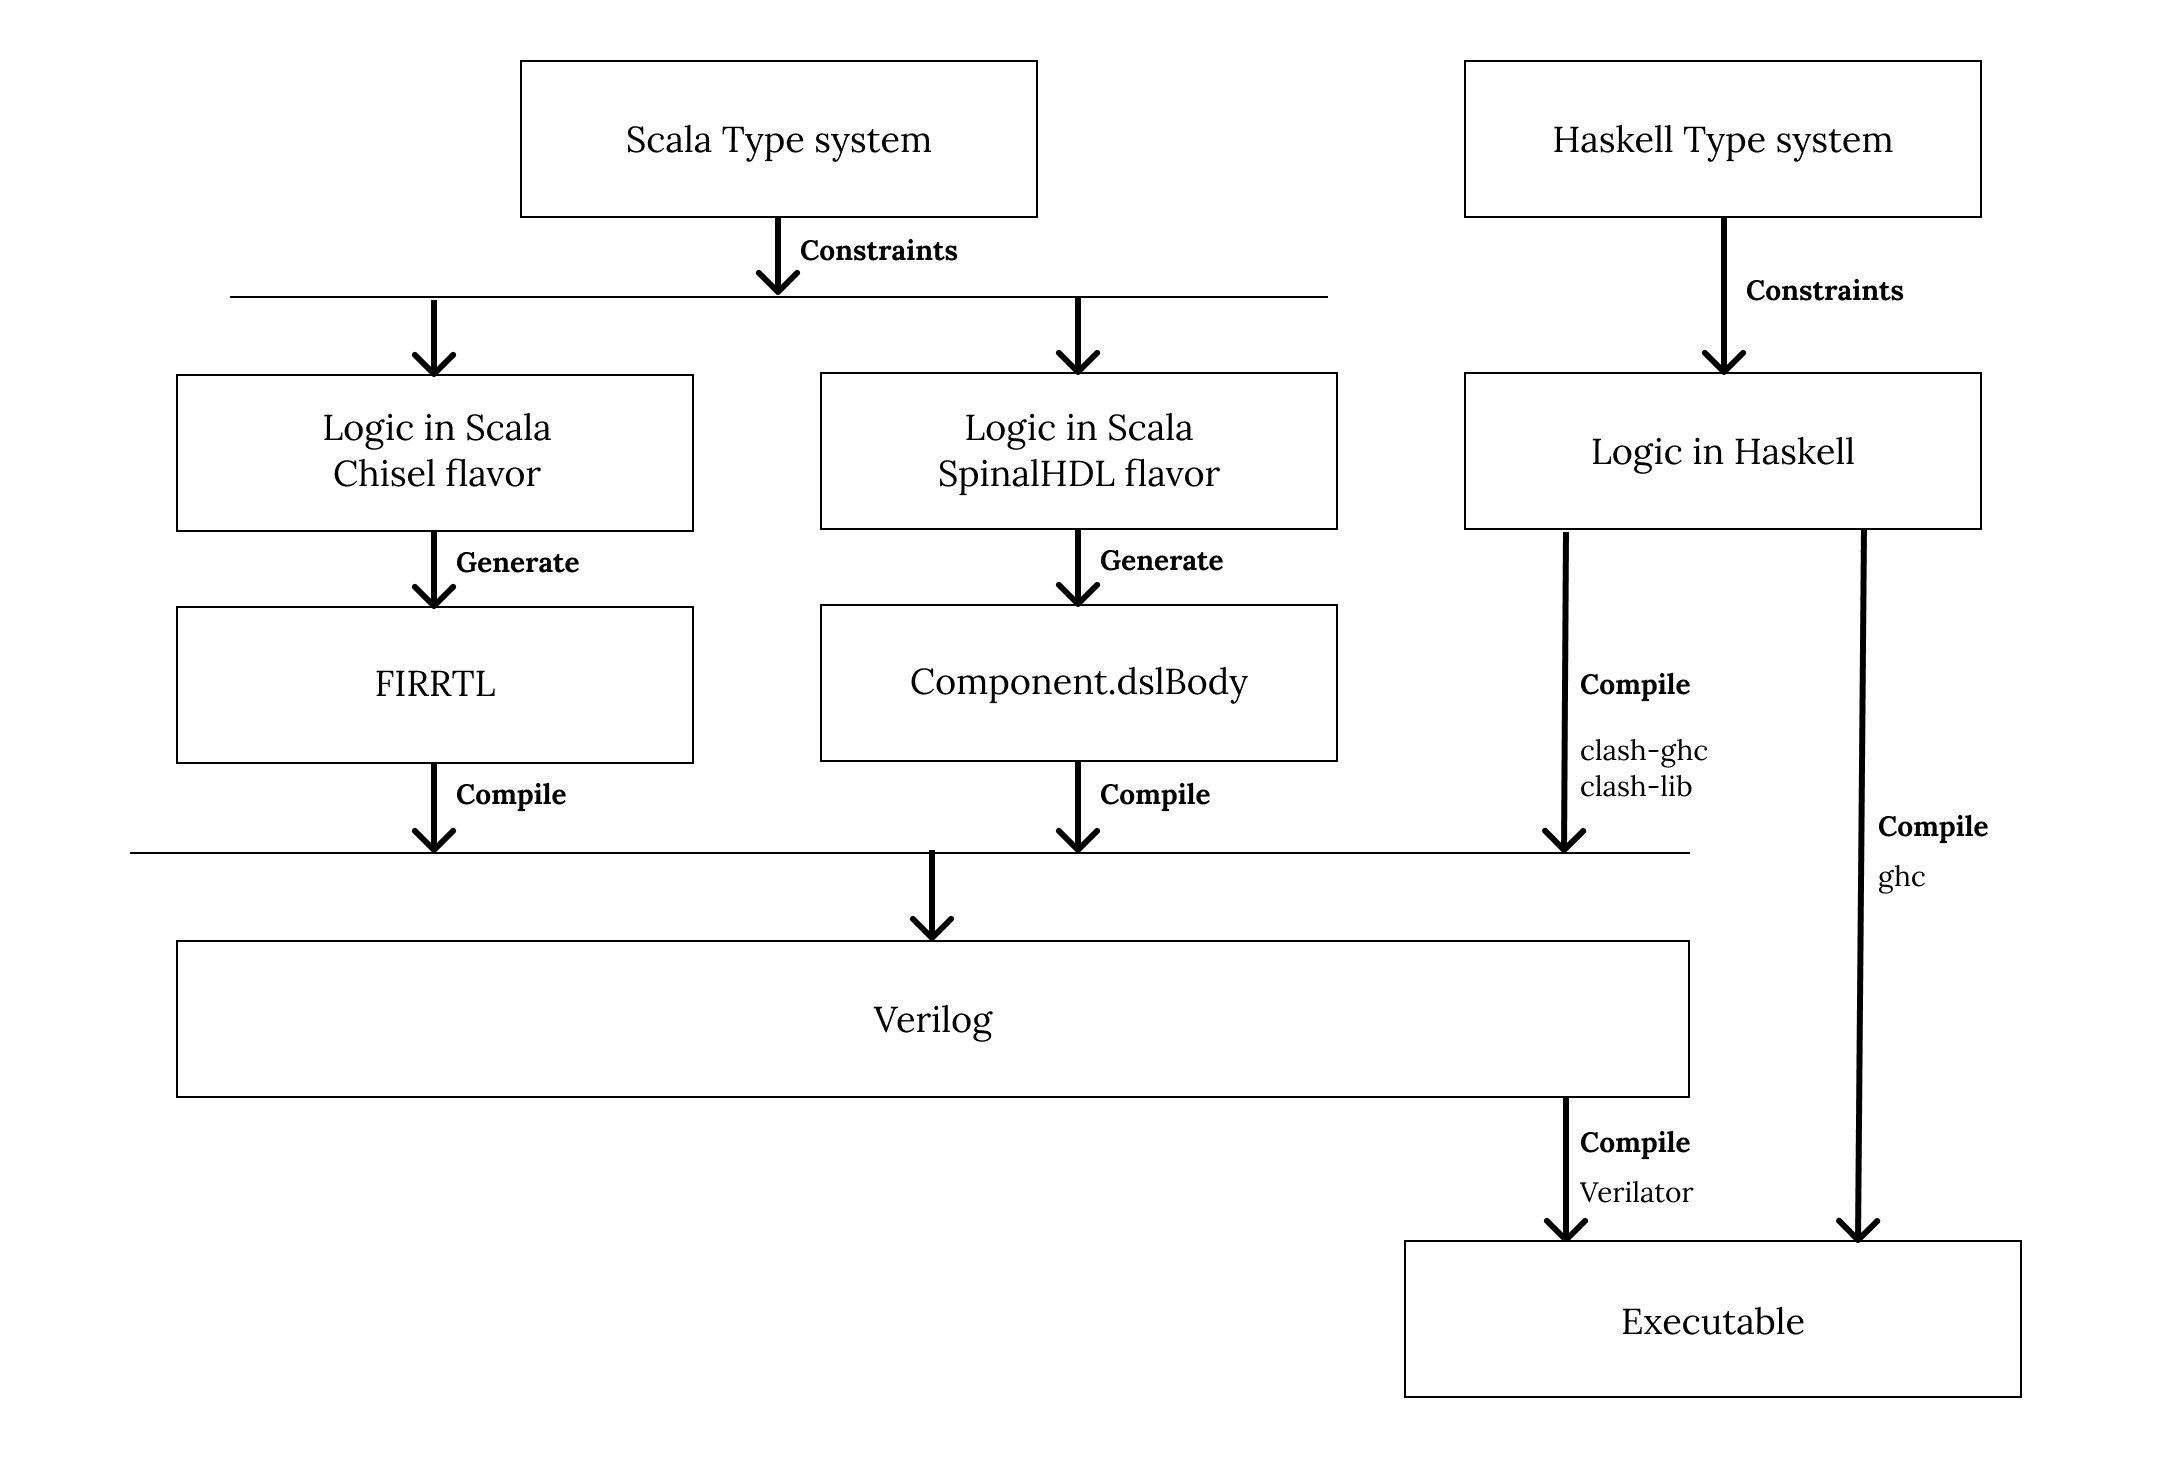
\includegraphics[width=0.8\textwidth]{Frame_1(3).png}
\caption{\label{fig:frame3}Scala-based shallowly-embedded HCLs need to, while Haskell-based deeply-embedded HCL Clash }
\end{figure}



\section{Verification Based On Cocotb\cite{rosser2018cocotb}}
\subsection{A Brief Introduction Of Cocotb}
Cocotb is a python-based testbench environment for verifying VHDL, Verilog, and SystemVerilog RTL designs\cite{cocotb_doc}. The framework of Cocotb-based verification can be divided into main parts: a python-based testbench that drives stimulus onto input ports and monitors output ports of DUT(DUT: Design Under Test ) and a simulator to simulate the hardware design. And the python testbench interacts with DUT in the simulation through standard VPI(VPI: Verilog Procedural Interface), VHPI(VHPI: VHDL Procedural Interface), or FLI(FLI: Foreign Language Interface) of the simulator. According to the principle of how it works, Cocotb can be used with any simulator that implements the industry-standard VPI, VHPI, or FLI interfaces, which means Cocotb can support most kinds of existing simulators ranging from commercial ones to open-source ones, including Iverilog, Verilator, Synopsys VCS, Mentor ModelSim and so on.

\begin{figure}[h]
\centering
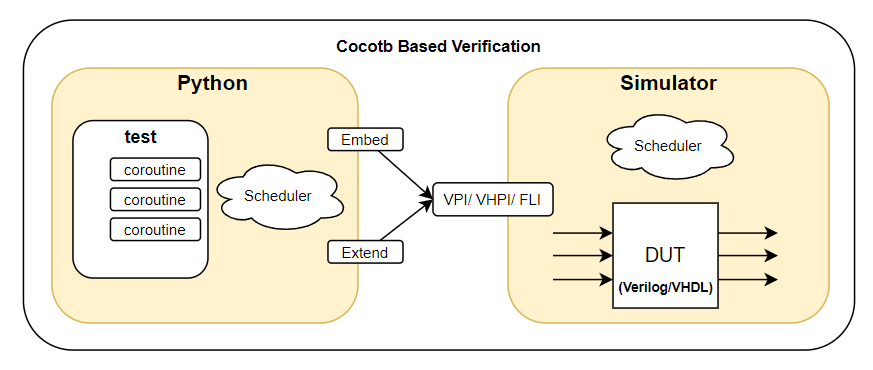
\includegraphics[width=0.52\textwidth]{cocotb.png}
\caption{\label{fig:coco}Cocotb based Verification framework}
\end{figure}

\subsection{Advantages Of Using Cocotb For Verification}
Besides its support for different kinds of simulators, Cocotb has various advantages over using Verilog, System Verilog, or VHDL for verification, which can accelerate the whole process of hardware design. Here are some significant advantages of Cocotb:

\subsubsection{Language Features Of Python}
\paragraph{}
Python is far more productive, expressive and succinct than traditional languages used for verification like Verilog, VHDL, and System Verilog. Compared to coding in these traditional  languages, it’s much easier for us to use python to implement a complicated function with less amount of codes. At the same time, Python has simple grammar and abundant online learning materials, making it more easier for novices to master. What’s more, Python is a high level programming language with many advanced features like object-oriented, which can help programmer produce more reusable codes.

In most cases of hardware verification, C/C++ is used to build reference models of DUTs and codes of reference models are integrated into SV(System Verilog) test codes through DPI. One of programming scenarios in which Python is far more efficient than other languages like C/C++ used in building reference model is arithmetic operations of big integers whose width is normally more than 64-bit. Algorithms in cryptography like ECC and RSA and hash functions usually involve operations of numbers of big width ranging from 128-bit to 2048-bit. The primitive types in C/C++ only support numbers of up to 64-bit. It's troublesome to deal with these big integers when using C/C++ to build your reference model. The C program below implements the addition of two big integers wider than 64-bit:
\begin{lstlisting}[language=C]
/* big_int_arith.h */
#ifndef BIG_INT_ARITH_H
#define BIG_INT_ARITH_H
#define MAX_SIZE 10
typedef struct big_int{
    int width;
    int numbers[MAX_SIZE];
} big_int;
big_int big_int_init(char input[]);
big_int big_int_add(big_int op1, big_int op2);
#endif
/* big_int_arith.c */
#include "big_int_arith.h"
#include <string.h>
big_int big_int_init(char input[]){
    big_int res;
    int len = strlen(input);
    res.width = len;
    if(len > MAX_SIZE) {res.width = MAX_SIZE;}
    for(int i=0; i<MAX_SIZE; i++){
        if(i < res.width){ res.numbers[i] = input[len-1-i] - '0';}
        else{ res.numbers[i] = 0;}
    }
    return res;
}

big_int big_int_add(big_int op1, big_int op2){
    int max = op1.width;
    if(max < op2.width) max = op2.width;
    for(int i; i< MAX_SIZE-1; i++){
        op1.numbers[i] += op2.numbers[i];
        op1.numbers[i+1] += op1.numbers[i]/10;
        op1.numbers[i] = op1.numbers[i]%10; 
    }
    op1.numbers[MAX_SIZE-1] += op2.numbers[MAX_SIZE-1];
    op1.numbers[MAX_SIZE-1] = op1.numbers[MAX_SIZE-1]%10;
    if(max == MAX_SIZE){ op1.width = max;}
    else{op1.width = (op1.numbers[max]==0)?max:max+1;}
    return op1;
}
\end{lstlisting}

Python implementation of addition operations on integers of any bit width:

\begin{lstlisting}[language=python]
# python implements addition of integers with any bit width
c = a + b
\end{lstlisting}

In C program, integers wider than 64-bit are stored in the format of array and arithmetic of these numbers like addition and multiplication needs to operate on every element of the array. However, integers in Python support any bit width and arithmetic symbols can be used to compute arithmetic operations of these big integers directly without additional codes. There are still many other cases in which Python can expedite the building of reference models and reduce the possibility of error. Although Python may fall slightly behind C/C++ in terms of performance, accuracy and efficiency are more important when it comes to hardware verification.

\subsubsection{Advantages Brought By Python Community}
\paragraph{}
Python is widely used in many programming scenarios and has multiple kinds of libraries or packages. With Cocotb, it’s straightforward to reuse these existing python-based algorithms or model implementations as the golden model of your hardware design. Or it’s also more convenient to build the reference model based on the existing python libraries or packages. For example, when designing accelerators for deep learning, python libraries like \textbf{Pytorch}, \textbf{Tensorflow}, and \textbf{Caffe} can be easily combined with Cocotb testbenches of your designs. And for verification of some complex bus protocols used for SoC integration such as AXI, PCIe, etc, Cocotb provides corresponding open-source libraries. Reusing the existing python library for building a golden model has two significant advantages: 
\begin{itemize}
    \item  ensure the correctness of the reference model or reduce the possibility of errors.
    \item avoid building every verification component from scratch and greatly reduce the workload.
\end{itemize}

\begin{figure}[hbt]
\centering
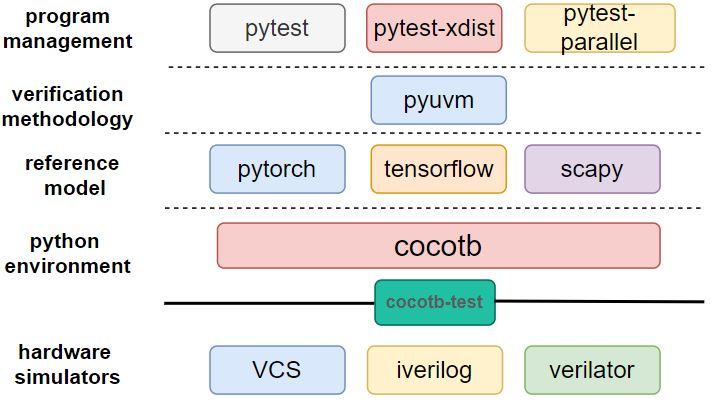
\includegraphics[width=0.58\textwidth]{cocotb-package.jpg}
\caption{\label{fig:cocotb}different packages used in cocotb verification}
\end{figure}

Besides facilitating the construction of reference models, there are many open-source python libraries and packages that can also help us write, organize and execute verification codes. It’s inevitable to interact with the simulator to execute our testbenches on it in the process of chip verification. Cocotb self provides a Makefile template to help developers interact with the simulator without using specific Linux commands. It’s still a little fussy to write and execute Makefile to get your codes running on the simulator. But \textbf{cocotb-test} package encapsulates the manipulations of the simulator and provides them as python functions to developers. By using \textbf{cocotb-test} package, users just need to call a python function and specify its parameters to start simulation, which provides standard python unit testing capabilities for \textbf{cocotb}. 

Based on the usage of \textbf{cocotb-test} package, you can write and manage test programs more efficiently by using \textbf{pytest}, a python package that implements mature full-featured Python testing tools. What’s more, you can also use \textbf{pytest-xdist} or \textbf{pytest-parallel} package for parallel run of your verification codes in multicore processors, which helps you make good use of computation ability to reduce execution duration. At the same time, package \textbf{pyuvm} has implemented main parts of UVM(UVM: Universal Verification Methodology) ,which is the most widely-used verification framework in industry. Based on \textbf{cocotb} and \textbf{pyuvm}, developers can use python instead of SystemVerilog to apply the methodology of UVM in their verification.

Verification is an indispensable and crucial part in the whole process of chip development especially in industry and it accouts for the most workload of a chip project. So there have been many attempts trying to improve the efficiency and speed of hardware verification. And \textbf{cocotb} is trying to provide a python environment or platform for verification. Based on this platform, you can enjoy the convenience brought by python’s succinct grammar and prosperous community, which will greatly accelerate the process of verification.

\subsection{A Specific Example of Cocotb}
\paragraph{}
In this part, a specific example of Cocotb-based verification is introduced and the design under test is a matrix multiplier implemented in System Verilog. The parameters and interface of DUT are listed in Table3 and Table4 respectively:
\begin{table}[h]
    \centering
    \caption{Parameters Of Matrix Multiplier Under Test}
    \begin{tabular}{|>{\raggedright\arraybackslash}m{3.8cm}|>{\raggedright\arraybackslash}m{2.2cm}|>{\raggedright\arraybackslash}m{7.8cm}|}
        \hline
         Parameter &  Default Value & Usage \\
         \hline
         DATA_WIDTH & 8 & Specify the width of input data \\
         \hline
         A_ROWS & 8 & Specify the number of rows of input matrix a \\
         \hline
         A_COLUMNS_B_ROWS & 4 & Specify the number of columns of a and rows of b \\
         \hline
         C_DATA_WIDTH & 18 & Specify the width of data in the output matrix c  \\ 
         \hline
    \end{tabular}
    \label{tab:my_label}
\end{table}

\begin{table}[h]
    \centering
    \caption{Interfaces Of The Matrix Multiplier Under Test}
    
    \begin{tabular}{|>{\centering\arraybackslash}m{1.5cm}|>{\centering\arraybackslash}m{1.8cm}|>{\raggedright\arraybackslash}m{8cm}|}
        \hline
         \textbf{Port} & \textbf{Direction} & \textbf{Width} \\
        \hline
         clk_i   & input  & 1 \\
        \hline
         reset_i & input  & 1 \\
        \hline
         valid_i & input  & 1 \\
        \hline
         valid_o & output &  1 \\
        \hline
         a_i & input & [DATA_WIDTH-1:0] [A_ROWS * A_COLUMNS_B_ROWS] \\
        \hline
         b_i & input & [DATA_WIDTH-1:0] [A_COLUMNS_B_ROWS * B_COLUMNS] \\ 
        \hline
         c_o & output & [C_DATA_WIDTH-1:0] [A_ROWS * B_COLUMNS]\\
        \hline
    \end{tabular}
    \label{tab:my_label}
\end{table}

\subsubsection{Build Reference Model}
\paragraph{}
The reference model of the matrix multiplier can be implemented based on numpy,  a well known python package which provides abundant matrix operations. Based on numpy, method “matmul” can be used to implement matrix multiplication directly and then there is no need to use loop syntax. The specific python implementation of the reference model is shown as below:
\begin{lstlisting}[language=python]
from typing import List
import numpy as np
class MatrixMultiplierTester:
    def __init__(self, target):
        self.dut = target
        self.buffer = Queue()
    
    def reference_model(self, input_a:List, input_b:List):
        array_a = np.array(input_a, dtype=np.uint64).reshape(A_ROWS, A_COLUMNS_B_ROWS)
        array_b = np.array(input_b, dtype=np.uint64).reshape(A_COLUMNS_B_ROWS, B_COLUMNS)
        array_c = np.matmul(array_a , array_b)
        array_c = array_c.reshape(-1)
        return array_c.tolist()

\end{lstlisting}

\subsubsection{Build Verification Platform}
\paragraph{}
The structure of a simple verification platform built on Cocotb is shown in the picture below. The verification platform mainly includes four parts: 1) driver; 2)monitor; 3) reference model; 4) buffer. The driver generates random input signals including  “valid_i”,“a_i”, and “b_i” using Python package \textbf{random}. When “valid_i” is high, the generated “a_i” and “b_i” are sent to the reference model and get the corresponding reference output. Reference outputs are stored in a buffer implemented through Python package \textbf{Queue} and once the output signal “valid_o” is high, the monitor samples output ports of DUT and compare their values with the reference output dequeued from buffer. The driver and monitor function are implemented as \textbf{coroutines} of Python, which is similar to multithreading and are executed concurrently.

\begin{figure}[h]
\centering
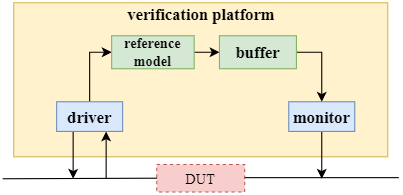
\includegraphics[width=0.5\textwidth]{verification_platform.png}
\caption{\label{fig:frame6} The Structure of a Cocotb-based Verification Platform}
\end{figure}

\subsubsection{Run Simulation}
\paragraph{}
The execution of verification codes based on Cocotb can be launched on simulators through Makefile without using commands to interact with simulators directly. Besides, by using method “simulator.run” provided in \textbf{cocotb-test} package, we can launch verification process in a python function directly. And then we can run the function directly or use \textbf{pytest}, a mature python test framwork, to manage the executions of all tests.

\begin{lstlisting}[language=python]
@pytest.mark.parametrize("data_width", [8,16])
def test_matrix_multiplier(data_width):
    module = "test_matrix_multiplier_2"
    toplevel = "matrix_multiplier"
    verilog_sources = ["./matrix_multiplier.sv"]
    parameters = {"DATA_WIDTH":data_width, "A_ROWS":10, "B_COLUMNS":4, "A_COLUMNS_B_ROWS":6}
    simulator.run(
        verilog_sources = verilog_sources,
        toplevel = toplevel,
        module = module,
        parameters = parameters
    )
\end{lstlisting}

Some pytest commands to manage executions of test units:
\begin{lstlisting}
# run all tests under current directory
  pytest

# execute tests in test_matrix_multiplier.py
# and enable printing log infomation
  pytest -o log_cli=True test_matrix_multiplier.py

# Run test in parallel (after installing pytest-xdist )
  pytest -n CPU_NUMS

# List all available tests under current directory
  pytest --collect-only

# execute tests in test_matrix_multiplier.py
# and display the output of print function
  pytest -s test_matrix_multiplier.py
\end{lstlisting}

\section{Conclusion}
\paragraph{}
In this article, we mainly talk about the design and verification of digital hardware based on the emerging and open-source tools including SpinalHDL and Cocotb, which we believe can innovate the traditional chip development process. The requirements for hardware design are becoming more and more various while there is no apparent improvement in design languages and tools. And what SpinalHDL and Cocotb is attempting to do is mainly about bringing some advanced and efficient concepts and methods of software desgin into the development flow of hardware. Compared to traditional design and verification methods based on System Verilog or VHDL, SpinalHDL and Cocotb can improve both the efficiency and quality of hardware development significantly.

It’s worth noting that SpinalHDL is not a new kind of HLS(HLS: High-Level Synthesis) instead it has the same description level as Verilog or VHDL. Combined with our development experience with Spinal, we summarize its three main advantages over Verilog and VHDL, including reliability, expressiveness and reusability. As for reliability, Spinal can provide more accurate abstraction of basic circuit elements, earlier check of some design rules during compilation, and separate design and simulation elements. And for expressiveness, SpinalHDL is built on Scala, a high level programming language. Based on Scala’s features including object-oriented, functional programming, recursion and abundant collection type, it’s more easier for hardware developers to implement and parameterize their designs. When it comes to reusability, SpinalHDL itself provides abundant encapsulation of frequently used circuit elements to reuse. And it’s also easier for designers to produce more reusable codes and build their own code base using Scala and its related toolchains. 

As for Cocotb, it has two main advantages over traditional verification tools. Similar to Scala, Python is a kind of high-level programming language with succinct grammar, great expressiveness, and some advanced language features, which greatly facilitates the verification of hardware design. And more importantly, Python is widely applied in many programming cases and has a strong and prosperous community. It’s much more convenient to build your verification based on existing abundant Python packages and libraries. 


\bibliographystyle{IEEEtran}  %格式
\bibliography{r1,r2,r3,r4}  %bib文件名

\end{document}